%%%%%%% Arquivo geral - recebe as informa��es dos preliminares, monta o sum�rio
%%%%%%% a lista de tabelas, a lista de figuras. � necess�rio entrar com arquivo de s�mbolos
%%%%%%% e abreveaturas. Recebe ainda as informa�oes do texto principal, refer�ncias 
%%%%%%% bibliogr�ficas e ap�ndices.
% A classe do documento est� definida em modelo.tex, bem como o layout da folha.

%%%%%%%%%%%%%%%%%%%%% pend�ncias:
%%%%%%%%%%%%%%%%%%%%% - tirar o negrito e os dois pontos das legendas de figuras e tabelas;
%%%%%%%%%%%%%%%%%%%%% - retirar os [ ] das refer�ncias nas refer�ncias e no caso das citacoes
%%%%%%%%%%%%%%%%%%%%% - substitu�-los por ( ).
%%%%%%%%%%%%%%%%%%%%% - retirar a palavra Ap�ndice do t�tulo dos nos Ap�ndices.


\documentclass[a4paper,12pt,oneside]{teseft}

\pagestyle{plain}

\usepackage{indentfirst} % Identar tamb�m o primeiro par�grafo de cada se��o

%\userpackage{}

%\usepackage[brazilian]{babel}
%\usepackage[utf8]{inputenc}
%\usepackage[T1]{fontenc}

\usepackage[brazil]{babel} % Suporte para o Portugu�s
\usepackage[utf8]{inputenc} % Suporte para acentua��o sem necessidade dos
% comandos especiais.
%\usepackage{mathrsfs} % estabelece fontes para it�lico em modo matem�tico
\usepackage{graphicx}
%\usepackage{flafter}
%\usepackage[all]{xy}
%\usepackage[none]{hyphenat} % N�o utiliza separa��o de s�labas.

%Dimens�es da p�gina ok
\paperwidth=210mm
\paperheight=297mm

%\voffset=-11.4mm % dist�ncia de 15mm ao topo da p�gina (1in+(-11.4mm)=14mm).
\voffset=-11.4mm
% topmargin - distancia acima do in�cio do cabe�alho (no caso 5 mm)
\topmargin=5mm
\headheight=0mm % topmargin, headheight e headsep totalizam 10mm, 
%que, somados aos 15mm 
%%%%%%%%%%%%%%%%% anteriores, resultam nos 25mm especificados para a margem superior.
\headsep=5mm 
% headsep - separa�ao vertical entre o cabe�alho e o in�cio do corpo do texto.
%\textheight=247mm % 297mm-2*25mm, ou seja, a altura da p�gina menos o espa�o reservado
%%%%%%%%%%%%%%%%%%% para as margens superior e inferior.
\textheight=247mm
%\footskip=12mm    % assim, sobram cerca de 25mm-12mm=13mm entre a numera��o de p�gina e
%%%%%%%%%%%%%%%%%%% a parte inferior do papel. 
\footskip=9mm

%\hoffset=-10.4mm % dist�ncia de 15mm � parte esquerda da p�gina.
\hoffset=-10.4mm % dist�ncia de 20mm � parte esquerda da p�gina.
%\oddsidemargin=10mm % que, somados aos 15mm anteriores, resultam nos 25mm especificados.
%\evensidemargin=10mm
\oddsidemargin=15mm
\evensidemargin=15mm

%\textwidth=155mm % 210mm-30mm-25mm (30mm lado esquerdo 25 lado direito).
%\textwidth - largura do texto
\textwidth=155mm

\marginparsep=0mm
\marginparwidth=0mm % n�o � reservado espa�o para notas de margem lateral.

%Espa�amento 1,5
\linespread{1.3}

%%%%%%%%%%%%%%%%%%%%%%%%%%% 


% o pacote gr�fico ainda nao foi acrescentado
%\usepackage[dvips]{graphics}

% estou acrescentando os comandos abaixo: sao necess�rios
% para os tipos de par�grafos adotados: sem identa�ao e com uma linha
% em branco entre cada um.
%\setlength{\parindent}{0pt}
%\setlength{\parskip}{0.7cm plus 0.5ex minus 0.2ex}
% 

\usepackage{enumerate}
%\usepackage{enumitem} 
\usepackage{graphicx,color}
\usepackage{booktabs}
\usepackage{listings}
\usepackage{multirow}
\usepackage[table]{xcolor}

\usepackage{xcolor}
\usepackage{stackengine}
\newlength\llength
\llength=1.38ex\relax



\newenvironment{joincode}  {\let\orighscode=\hscode
  \let\origendhscode=\endhscode
  \def\endhscode{\def\hscode{\endgroup\def\@currenvir{hscode}\\}\begingroup}
    \orighscode\def\hscode{\endgroup\def\@currenvir{hscode}}}  {\origendhscode
  \global\let\hscode=\orighscode
  \global\let\endhscode=\origendhscode}

\newcommand{\neoidl}{NeoIDL}
\newcommand{\neocortex}{NeoCortex}
\newcommand{\bnfc}{\texttt{BNFConverter}}
\newcommand{\designbycontract}{\textit{Design-by-Contract}}
\newcommand{\twisted}{\textit{Twisted}}
\newcommand{\ws}{\textit{Web Service}}
\newcommand{\wss}{\textit{Web Services}}
\newcommand{\CdFirst}{\textit{Code-first}}
\newcommand{\CtFirst}{\textit{Contract-first}}
\newcommand{\framework}{\textit{framework}}
\newcommand{\method}[1]{\texttt{#1}}

\newcommand{\emptyP}{\mbox{$\epsilon$}}
\newcommand{\terminal}[1]{\mbox{{\texttt {#1}}}}
\newcommand{\nonterminal}[1]{\mbox{$\langle \mbox{{\sl #1 }} \! \rangle$}}
\newcommand{\arrow}{\mbox{::=}}
\newcommand{\delimit}{\mbox{$|$}}
\newcommand{\reserved}[1]{\mbox{{\texttt {#1}}}}
\newcommand{\literal}[1]{\mbox{{\texttt {#1}}}}
\newcommand{\symb}[1]{\mbox{{\texttt {#1}}}}


\definecolor{light-gray}{gray}{0.85}
\definecolor{dark-yellow}{RGB}{215,167,0}

\newcommand{\hilight}[1]{\colorbox{light-gray}{#1}}



\hyphenation{NeoIDL}

\lstdefinelanguage{json}{
  basicstyle=\normalfont\ttfamily,
  numbers=left,
  numberstyle=\scriptsize,
  stepnumber=1,
  numbersep=8pt,
  showstringspaces=false,
  breaklines=true,
  frame=top,
   literate=
  *{0}{{{\color{numb}0}}}{1}
  {1}{{{\color{numb}1}}}{1}
  {2}{{{\color{numb}2}}}{1}
  {3}{{{\color{numb}3}}}{1}
  {4}{{{\color{numb}4}}}{1}
  {5}{{{\color{numb}5}}}{1}
  {6}{{{\color{numb}6}}}{1}
  {7}{{{\color{numb}7}}}{1}
  {8}{{{\color{numb}8}}}{1}
  {9}{{{\color{numb}9}}}{1}
  {:}{{{\color{punct}{:}}}}{1}
  {,}{{{\color{punct}{,}}}}{1}
  {\{}{{{\color{delim}{\{}}}}{1}
  {\}}{{{\color{delim}{\}}}}}{1}
  {[}{{{\color{delim}{[}}}}{1}
  {]}{{{\color{delim}{]}}}}{1},
}



\lstdefinelanguage{NeoIDL}{
  sensitive = true,
  keywords={},
  otherkeywords={% Operators
    >, <, ==
  },
  keywords = [2]{module, resource, enum, annotation, for, import, entity, path,
  @get, @post, @put, @delete, require, ensure, otherwise, call, and, or, not},
  keywordstyle=[1]\color{dark-yellow}\textbf,
  keywordstyle=[2]\color{black}\textbf,
  numbers=left,
  numberstyle=\scriptsize,
  stepnumber=1,
  numbersep=8pt,
  showstringspaces=false,
  breaklines=true,
  frame=top,
  comment=[l]{//},
  morecomment=[s]{/*}{*/},
  commentstyle=\color{purple}\ttfamily,
  stringstyle=\color{red}\ttfamily,
  morestring=[b]',
  morestring=[b]"
  }

\lstdefinelanguage{PythonTwisted}{
  sensitive = true,
  keywords = {classe, object, def, return},
  numbers=left,
  numberstyle=\scriptsize,
  stepnumber=1,
  numbersep=8pt,
  showstringspaces=false,
  breaklines=true,
  frame=lines,
  comment=[l]{\#},
  morecomment=[s]{/*}{*/},
  commentstyle=\color{purple}\ttfamily,
  stringstyle=\color{red}\ttfamily,
  morestring=[b]',
  morestring=[b]"
  }
  

\lstdefinelanguage{Haskell}{
  sensitive = true,
  keywords = {data, type, module, where, do, IO, import},
  numbers=left,
  numberstyle=\scriptsize,
  stepnumber=1,
  numbersep=8pt,
  showstringspaces=false,
  breaklines=true,
  frame=lines,
  }
  
  \lstdefinelanguage{HaskellSimple}{
  sensitive = true,
  keywords = {data, type, module, where, do, IO, import},
  showstringspaces=false,
  breaklines=true,
  frame=lines,
  }
  
  \lstdefinelanguage{Eiffel}{
  sensitive = true,
  keywords = {class, feature, create, require, ensure, end, is, INTEGER,
  requires, ensures}, numbers=left,
  numberstyle=\scriptsize,
  stepnumber=1,
  numbersep=8pt,
  showstringspaces=false,
  breaklines=true,
  frame=top,
  }
  

  \lstdefinelanguage{JML}{
  sensitive = true,
  keywords = {class, public, static, int, return},
  numbers=left,
  numberstyle=\scriptsize,
  stepnumber=1,
  numbersep=8pt,
  showstringspaces=false,
  breaklines=true,
  frame=top,
  }
  
   \lstdefinelanguage{SpecSharp}{
  sensitive = true,
  keywords = {class, public, require, ensure, true, int},
  numbers=left,
  numberstyle=\scriptsize,
  stepnumber=1,
  numbersep=8pt,
  showstringspaces=false,
  breaklines=true,
  frame=top,
  }
  
   \lstdefinelanguage{Perl}{
  sensitive = true,
  keywords = {use, my, split, local, undef, open, die, binmode, close, print,
  lc, if, exists, else, for keys, exists}, numbers=left,
  numberstyle=\scriptsize,
  stepnumber=1,
  numbersep=8pt,
  showstringspaces=false,
  breaklines=true,
  frame=top,
  }
  


\begin{document}
\pagenumbering{roman}
%\frontmatter
\thispagestyle{empty}

\begin{bf}
\hspace{10mm}
\vfill

\begin{center}
\rule{155mm}{0.1mm}

T�TULO DA DISSERTA��O EM MAI�SCULAS

\vspace{10mm}

AUTOR DA DISSERTA��O

\vspace{15mm}

DISSERTA��O DE MESTRADO EM ENGENHARIA EL�TRICA

\vspace{10mm}

DEPARTAMENTO DE ENGENHARIA EL�TRICA

\rule{155mm}{0.1mm}
\end{center}

\hspace{10mm}
\vfill
\end{bf}

\pagebreak

\thispagestyle{empty}
\hspace{10mm}

\pagebreak
 Uma capa semelhante a esta dever� ser usada na encaderna��o.


%=======================================================================
% Folha de t�tulo da disserta��o

\thispagestyle{empty}
\setcounter{page}{1}
\begin{center}
{\normalsize {\bf UNIVERSIDADE DE BRAS\'{I}LIA\\
FACULDADE DE TECNOLOGIA\\
DEPARTAMENTO DE ENGENHARIA EL\'{E}TRICA }}

\vfill

% INSERIR AQUI O T�TULO DA DISSERTACAO
{\large {\bf  CONTRATOS REST ROBUSTOS E LEVES: UMA ABORDAGEM EM
DESIGN-BY-CONTRACT COM NEOIDL }}


\vfill

% INSERIR AQUI O NOME DO AUTOR DA DISSERTA��O
{\large {\bf LUCAS FERREIRA DE LIMA}}

\vspace{20mm}

% INSERIR AQUI O NOME DO ORIENTADOR: (NOME)
{\normalsize {\bf ORIENTADOR: RODRIGO BONIFÁCIO DE ALMEIDA }}

\vspace{20mm}

{\normalsize {\bf DISSERTAÇÃO DE MESTRADO EM\\
% INSERIR ABAIXO O NOME DO PROGRAMA DE P�S-GRADUACAO
ENGENHARIA ELÉTRICA  }}

\vspace{10mm}

% inserir o n�mero da publica��o distinguindo entre disserta�ao (DM) e tese (TD)
{\normalsize {\bf PUBLICAÇÃO: MTARH.DM - 017 A/99 }}


\vspace{10mm}

% inserir o local, m�s e ano da publica�ao
{\normalsize {\bf BRASÍLIA/DF: JULHO - 2016.    }  }
\end{center}

\pagebreak

\thispagestyle{empty}
\hspace{10mm}
\addtocounter{page}{-1}

\pagebreak

%=======================================================================

\begin{bf}
\begin{center}
{\normalsize UNIVERSIDADE DE BRASÍLIA}\\
{\normalsize FACULDADE DE TECNOLOGIA}\\
% inserir nome do departamento
{\normalsize DEPARTAMENTO DE ENGENHARIA ELÉTRICA}\\

\vspace{10mm}
% inserir o nome da disserta�ao/tese
{\large {\bf  CONTRATOS REST ROBUSTOS E LEVES: UMA ABORDAGEM EM
DESIGN-BY-CONTRACT COM NEOIDL }}

\vspace{10mm}
% inserir nome do autor
{\large {\bf LUCAS FERREIRA DE LIMA}}
\end{center}
\end{bf}

\vspace{10mm}

\noindent\MakeUppercase{ {\bf
Dissertação de Mestrado submetida ao
% inserir nome do departamento
Departamento de Engenharia Elétrica
%%%%%%%%
da Faculdade de Tecnologia da Universidade de Brasília,
como parte dos requisitos necessários para a obtenção do grau de mestre em
% nome do Programa de p�s-gradua�ao
ENGENHARIA ELÉTRICA. }}

\vspace{5mm}

\noindent\MakeUppercase{ {\bf Aprovada por:}}

\vspace{10mm}

\begin{bf}
\noindent\rule{120mm}{0.1mm}\\
{ Prof. Rodrigo Bonifácio de Almeida, DSc. (ENE-UnB) }\\
{(Orientador)}

\vspace{7.5mm}

\noindent\rule{120mm}{0.1mm}\\
{ Prof. Rafael Timóteo de Sousa Jr., DSc. (ENE-UnB) }\\
{(Examinador Interno)}

\vspace{7.5mm}

\noindent\rule{120mm}{0.1mm}\\
{  Prof. Henrique Emanuel Mostaert Rebêlo, DSc. (UFPE) }\\
{(Examinador Externo)}

\vspace{7.5mm}
%%%%% outros membros, se houver
%\noindent\rule{110mm}{0.1mm}\\
%{(Titula��o do examinador externo) Nome do examinador externo}\\
%{(Examinador Externo)}

\vspace{7.5mm}
%local e data
\noindent\MakeUppercase{Brasília/DF, 11 DE JULHO DE 2016.}
\end{bf}

\pagebreak

%\thispagestyle{empty}
%\hspace{10mm}
%\addtocounter{page}{-1}

%\pagebreak

%

\noindent \begin{bf} \MakeUppercase{Ficha Catalográfica} \end{bf}

% \vspace{10mm}

\noindent\framebox[155mm][l]{\begin{tabular}{l}
% inserir  NOME DO AUTOR (�ltimo nome seguido de v�rgula e dos primeiros nomes)
  \hspace{2mm}  LIMA, LUCAS FERREIRA DE \\
  % t�tulo da disserta�ao (identar o resto do t�tulo em 21 mm, caso o mesmo nao
  % caiba em uma linha), acrescentar [Distrito Federal] e o ano. 
   \hspace{2mm} Contrato REST robustos e leves: uma abordagem em
   Design-by-Contract\\ com NeoIDL.
   [Distrito Federal] 2016.\\
%  numero de paginas de preliminares e texto, tamanho da p�gina e outros dados padroes.
  \hspace{2mm} xvii, 98p., 297 mm (ENE/FT/UnB, Mestre, Engenharia Elétrica,
  2016).  \\
  \hspace{2mm} Dissertação de  Mestrado - Universidade de Brasília. \\
  \hspace{2mm} Faculdade de Tecnologia. \\
%  
 % nome do departamento
  \hspace{2mm}  Departamento de Engenharia Elétrica. \\
    % palavra-chave 1
  \begin{tabular}{ll}
  \hspace{1mm}  1. Computação orientada a serviços  & 
  % palavra-chave 2
    ~ ~ ~ ~ ~ 2. \designbycontract{}\\
  % palavra-chave 3  
  \hspace{2mm}3. \neoidl{}
  %palavra-chave 4
  & ~ ~ ~ ~ ~ 4. REST \\
  % texto padrao
  \hspace{2mm}I. ENE/FT/UnB &~ ~ ~ ~ ~ II. Título (série) \end{tabular}
  \end{tabular}}

  
\vspace{10mm}

\noindent \begin{bf} \MakeUppercase{Referência Bibliográfica} \end{bf}

\vspace{-1mm}

\noindent CONTRATOS REST ROBUSTOS E LEVES: UMA ABORDAGEM EM
DESIGN-BY-CONTRACT COM NEOIDL

% refer�ncia bibliogr�fica padrao para o autor
\noindent  LIMA, L. F. (2016). Contratos REST Robustos e Leves: Uma
Abordagem em Design-by-Contract com NeoIDL. Dissertação de Mestrado em
Engenharia Elétrica, Publicação 642/2016 DM PPGEE, Departamento de Engenharia Elétrica,
Universidade de Brasília, Brasília, DF, 82p.



\vspace{6mm}

\noindent \begin{bf} \MakeUppercase{Cessão de Direitos} \end{bf}

\vspace{5mm}

% nome do autor
\noindent NOME DO AUTOR: Lucas Ferreira de Lima.
\vspace{6mm}

% t�tulo da dissertacao
\noindent TÍTULO DA DISSERTAÇÃO DE MESTRADO: Contratos REST Robustos e Leves: Uma
Abordagem em Design-by-Contract com NeoIDL. 

\vspace{3mm}
% grau e ano
\noindent GRAU / ANO:~ ~ ~ Mestre / 2016

\vspace{5mm}

\noindent É concedida a Universidade de Brasília permissão para reproduzir
cópias desta dissertação de mestrado e para emprestar ou vender tais cópias
somente para propósitos acadêmicos e científicos. O autor reserva outros
direitos de publicação e nenhuma parte desta dissertação de mestrado pode ser
reproduzida sem a autorização por escrito do autor.

\vspace{5mm}

\noindent \underline{\hspace{65mm}}

\vspace{-2mm}
% nome do autor

\noindent  Lucas Ferreira de Lima
   \vspace{-2mm}

 % endere�o do autor
\noindent Cond. RK Conj. Antares Qd. L Cs. 48 Sobradinho 
    \vspace{-2mm}
    
\noindent 73.252-200 - Brasília - DF - Brasil.

\pagebreak

% p�gina em branco a seguir, sem numera�ao (empty)
%\thispagestyle{empty}
%\hspace{10mm}
%\addtocounter{page}{-1}

%\pagebreak

%\vspace{5mm}

\noindent {\large \begin{bf} \MakeUppercase{Dedicatória} \end{bf}}

\vspace{13cm}



\begin{quote}
  \hspace{7cm} Este trabalho é dedicado a ...\\ 
  
  \vspace{-10mm}
   \hspace{7cm}   continuação ............ 
\end{quote}


\clearpage
\pagebreak

% p�gina em branco a seguir, sem numera�ao (empty)
%\thispagestyle{empty}
%\hspace{10mm}
%\addtocounter{page}{-1}

%\pagebreak

%\vspace{5mm}

\noindent {\large \begin{bf} \MakeUppercase{Agradecimentos} \end{bf}}

%\vspace{3cm}

\begin{quote}

Agradeço a Deus, pela fé e esperança para superar as adversidades.\\
A minha amada esposa Paula, pelo imenso companherismo, estímulo e por ter se
desdobrado nos momentos de minha ausência, em especial nos cuidados com nossas jóias
preciosas, nossos amados filhos João Filipe, Maria Luísa e Ana Júlia.\\
Aos meus pais, pela dedicação e carinho. Aos meus irmãos pelo exemplo
determinante. Ao suporte indispensável de minha sogra e sogro, cunhados e
sobrinhos.\\
Aos professores Rodrigo Bonifácio e Edna Canedo, pela orientação,
paciência, incentivo e aprendizado.\\
Aos professores Rafael Timóteo, Ricardo Puttini e Valério Aymoré, pelas
relevantes contribuições do conhecimento transmitido.\\
À equipe do TSE, pelo estímulo, colaboração, compreensão. Devo muito a vocês.\\
Aos professores da Universidade do Rio Grande no Norte, na pessoa do professor
Uirá Kulesza.\\
Aos professores coordenadores André Noll, Ugo Dias e Kleber Melo, e à
Adriana Reis e ao Igor pelo suporte no PPGEE.\\
Aos oficiais do exército brasileiro, na pessoa do Thiago Mael, pela enorme
colaboração e crítica técnica. Nota de destaque para Leandro Loriato, pelas
questões importantes debatidas.\\
À equipe da Secretaria de Orçamento Federal, na pessoa do Marcos
César.\\


% Deus
% Família (pais, irmãos, esposa, filhos, cunhados e todos os outros)
% Professores Rodrigo, Edna, Uirá - orientação
% Professores Rafael, Puttini e Paulo 
% Coordenadores André Noll, Ugo Dias e Kleber Melo 
% Apoio: Adriana Reis e Igor 
% Equipe do Exército, na pessoa do Thiago Mael, com destaque para Leandro
% Loriato
% Equipe da SOF, na pessoa do Marco
% Equipe do TSE

 
\end{quote}

\clearpage

\pagebreak

% p�gina em branco a seguir, sem numera�ao (empty)
%\thispagestyle{empty}
%\hspace{10mm}
%\addtocounter{page}{-1}

%\pagebreak


%%%%%%%%%%%%%%%%%%%%%%%%%%% Resumo e abstract %%%%%%%%%%%%%%%%%%%%%%%%
\noindent {\large {\bf RESUMO}}

\vspace{5mm}

\noindent {\bf CONTRATOS REST ROBUSTOS E LEVES: UMA ABORDAGEM EM
DESIGN-BY-CONTRACT COM NEOIDL } 
 
\vspace{5mm} 

\noindent  {\bf
Autor: Lucas Ferreira de Lima}

\noindent {\bf Orientador: Rodigo Bonifácio de Almeida}

\noindent {\bf Programa de Pós-Graduação em Engenharia Elétrica}

\noindent {\bf Brasília, julho de 2016 }

\vspace{5mm}
\noindent
A adoção do paradigma arquiteturação baseado em serviços\ldots 
O presente trabalho foi desenvolvido, \ldots, tendo como 
objetivo geral .................... Como objetivos específicos, o trabalho
procurou .........

\vspace{5mm}
\noindent
A proposta partiu\ldots

\vspace{5mm}
\noindent
Durante a realização\ldots

\vspace{5mm}
\noindent
Os resultados sugerem\ldots



  
\clearpage




\noindent
{\large {\bf ABSTRACT}}

\vspace{5mm}
\noindent {\bf CONTRATOS REST ROBUSTOS E LEVES: UMA ABORDAGEM EM
DESIGN-BY-CONTRACT COM NEOIDL } 
 
\vspace{5mm} 

\noindent  {\bf
Autor: Lucas Ferreira de Lima}

\noindent {\bf Orientador: Rodigo Bonifácio de Almeida}

\noindent {\bf Programa de Pós-Graduação em Engenharia Elétrica}

\noindent {\bf Brasília, julho de 2016 }

\vspace{5mm}
\noindent
..

\vspace{5mm}
\noindent
..

\vspace{5mm}
\noindent
..

\vspace{5mm}
\noindent
..

\clearpage

%%%%%%%%%%%%%%%%%%%%%%%%%%% 

%
\tableofcontents
\listoftables
\listoffigures

\pagebreak

% \clearpage
%\hspace{1pt}\vspace{1pt}
%\pagebreak
\noindent {\large \begin{bf} LISTA DE S\'{I}MBOLOS, NOMENCLATURA E
ABREVIAÇÕES
\end{bf}}
%\addcontentsline{toc}{chapter}{LISTA DE S�MBOLOS, NOMECLATURAS E ABREVIA��ES}

\newcommand{\acrlista}[1]{\vspace{12pt}\noindent #1\\}
\newcommand\tab[1][1cm]{\hspace*{#1}}


\begin{table}[!bth] 
\begin{tabular}{p{2cm}p{13cm}}
API & Application Programming Interface\\
BPM & Business Process Modeling\\
DbC & \designbycontract{}\\
DSL & Domain Specific Language\\
EAI & Interface Description Languages \\
Eiffel & Linguagem de programação orientada a objetos com suporte a
DbC\\
GQM & Goals-Questions-Metrics\\
JML & Java Modeling Language\\
NeoCortex & Framework de serviços do Exército Brasileiro\\
NeoIDL & Linguagem e framework para especificação e geração de serviços REST\\
Twisted & Um framework orientado a eventos de rede escrito em Python\\
RAML & RESTful API Modeling Language\\
REST & Representational State Transfer\\
SOA & Software Oriented Architecture\\
SOC & Software Oriented Computing\\
Spec\# & Extensão de linguagem C\# para \designbycontract{}\\
Swagger & Open RESTful API Representation Language\\
TAM & Technology Acceptance Model\\
TI & Tecnologia da Informação\\
URI & Uniform Resource Identifier\\
WSDL & Web-services description language\\

\end{tabular}
\end{table}

\pagebreak


% fim do preambulo (preliminares) - a numera�ao a partir daqui � em ar�bico
% e come�ando da p�gina 1.

%%%%%%%%%%%%%%%%%% in�cio dos cap�tulos

% os dois comandos abaixo tiram a identa�ao nos par�grafos
% e indicam que o espa�o equivalente a uma linha de texto deve ser 
% deixado em branco entre par�grafos.
\setlength{\parindent}{0pt}
\setlength{\parskip}{0.7cm plus 0.5ex minus 0.2ex}
%

% Introdução - Estudos empíricos / DbC para NeoIDL
% Fundamentação teórica -
% NeoIDL - Objetivos / Resultados / Extensão da Linguagem / Avaliação empírica
% / Destacar as mudanças da sintaxe da NeoIDL para e o uso do BNFConverter
% Análise da Aceitação da NeoIDL - Método / GQM / Resultados
% Conclusão 

% 1. Introdução - DbC para SOC(NeoIDL), estudo empíricos


%%%%%%%%%%%%%%%%%% in�cio dos cap�tulos
% cap�tulo 1
\chapter{INTRODUÇÃO}
\pagenumbering{arabic}
\vspace{-6mm}

A computação orientada a serviços ( \emph{Service-oriented computing, SOC)} tem
se mostrado uma solução de \textit{design} de \textit{software} que favorece o
alinhamento às mudanças constantes e urgentes nas instituições
\cite{chen2008towards}. Nessa abordagem, os recursos de software são empacotados
como serviços, módulos bem definidos e auto-contidos, que provêem
funcionalidades negociais e com independência de estado e contexto
\cite{papazoglou2007service}.

Os benefícios de SOC estão diretamente relacionados ao
baixo acoplamento dos serviços que compõem a solução, de forma que as partes
(nesse caso serviços) possam ser subs\-ti\-tu\-í\-das e evoluídas facilmente, ou
ainda rearranjadas em novas composições. Contudo, para que isso seja possível, é
necessário que os serviços possuam contratos bem escritos e independentes da
implementação.

A relação entre quem provê e quem consome o serviço se
dá por meio de um contrato. O contrato de serviço é o documento que descreve os
propósitos e as funcionalidades do serviço, como ocorre a troca de mensagens,
informações sobre as operações e condições para sua execução \cite{erl2009web}.

Nesse contexto, a qualidade da especificação do contrato é fundamental para o
projeto de software baseado em SOC. Este trabalho de pesquisa aborda um aspecto
importante para a melhoria da robustez de contratos de serviços: a construção de
garantias mútuas por meio da especificação formal de contratos, agregando o
conceito de \designbycontract{} \cite{meyer1992applying}.

\section{PROBLEMA DE PESQUISA}
\vspace{-6mm}

As linguagens de especificação de contratos para SOC apresentam
algumas limitações. Por exemplo, a linguagem WSDL (\emph{Web-services
description language}) \cite{WSDLSite} é considerada uma solução
pouco expressiva pois se utiliza da notação XML e muitas marcações
(\textit{tags}) para descrever um contrato de \ws{}. Essa característica
desestimula a abordagem \textit{Contract First}.
Por essa razão, especificações WSDL são usualmente derivadas a partir de anotações em código
fonte (\textit{Code First}).
Além disso, os conceitos descritos em contratos na linguagem WSDL não são
diretamente mapeados aos elementos que compõem as interfaces do estilo
arquitetural REST\cite{fielding2000architectural} (\emph{Representational State Transfer}).

Outras alternativas para REST, como Swagger\cite{swaggerSite} e
RAML\cite{RAML}, usam linguagens de propósito geral (em
particular JSON\cite{JSon} e YAML\cite{YAML}) adaptadas para especificação de
contratos.
Ainda que façam uso de contratos mais sucintos que WSDL, essas linguagens não se
beneficiam da clareza típica das linguagens específicas para esse fim (como
a IDL\footnote{Interface Description
Languages.} CORBA\cite{corba}) e não oferecem
mecanismos semânticos de extensibilidade (capacidade de extender uma
especificação principal e agregar outros componentes) e modularidade
(especificação do contrato em partes separadas e reusáveis).

Com o objetivo de mitigar esses problemas, a linguagem \neoidl{} foi proposta
para simplificar a especificação de serviços REST com mecanismos de modularização,
suporte a anotações, herança em tipos de dados definidos pelo desenvolvedor, e
uma sintaxe simples e concisa semelhante às IDLs presentes em \emph{Apache
Thrift}\texttrademark\cite{thrift} e \emph{CORBA}\texttrademark\cite{corba}.

Por outro lado, a \neoidl{}, da mesma forma que WSDL,
Swagger e RAML não oferece construções para especificação de contratos formais
com aspecto comportamental como os presentes em linguagens que
suportam DbC (\emph{Design by Contract})~\cite{meyer1992applying}, como
Eiffel\cite{meyer1988eiffel}, JML\cite{leavens2006design} e
Spec\#\cite{barnett2004spec}. Em outras palavras, a \neoidl{} admite apenas contratos fracos (\textit{weak contracts}), sem suporte a construções com pré e
pós-condições.



\section{OBJETIVO GERAL}
\label{ObjGeral}
\vspace{-6mm}

O objetivo geral deste trabalho é investigar o uso de construções de
\designbycontract{} no contexto de computação orientada a serviços, verificando a
viabilidade e utilidade de sua adoção na especificação de contratos e
implementação de serviços REST. Para atingir o objetivo geral, os seguintes 
objetivos específicos foram definidos, sendo diretamente mapeados nas 
principais contribuições do trabalho. 

%\subsection{Objetivos específicos}
\vspace{-6mm}

\begin{enumerate}[(OE1)]
  \item Realizar análise empírica de expressividade e reuso da especificação de
  contratos em \neoidl{} em comparação com \textit{Swagger}, a partir de contratos
  reais do Exército Brasileiro (Seção \ref{EstudoExpressividadeReuso}); 
  \item Extender a sintaxe da \neoidl{} para admitir construções de 
  \designbycontract, com pré e pós-condições para operações de serviços REST
  (Seção \ref{extensaoNeoIDL-DbC});
  \item Incorporar à infraestrutura de \textit{Plugins} da
  \neoidl{} a capacidade de geração de código para o \framework{} \textit{Python
 Twisted} (Seção \ref{pluginTwisted});
  \item Implementar regras de transformação que traduzem construções de DbC
 \neoidl{} em código de validação para o framework \textit{Python
 Twisted} (Seção \ref{pluginTwisted});% com suporte a \designbycontract{} a
 % partir de contratos especificados em \neoidl;
  \item Coletar a percepção de desenvolvedores sobre a aceitação da
  especificação de contratos REST com \designbycontract{} na \neoidl{} (Seção
  \ref{analiseSubjetiva}).
\end{enumerate}


\section{JUSTIFICATIVA E RELEVÂNCIA}
\label{JustificativaRelevancia}
\vspace{-6mm}

A demanda por integração entre sistemas de várias origens e tecnologias diversas
fez aumentar a adoção de soluções baseada em computação orientada a serviços.
Isso se deve justamente à necessidade de tornar a interoperabilidade de soluções
heterogênias o menos acopladas possível, de modo que mudanças nos requisitos de negócio ou
na inclusão de novos serviços sejam atendidas com simplicidade,
eficiência e rapidez.

O uso de \ws{}\cite{erl2009web} é a forma mais comum de se implementar os serviços. O
desenvolvimento de \ws{}, que eram inicialmente projetados sobre a abordagem
SOAP, com o tráfego de mensagens codificadas em XML\cite{XML}, tem gradativamente
se intensificado no sentido da utilização de REST\cite{fielding2000architectural}.

Um dos principais benefícios do uso de SOC está na possibilidade de reuso de
seus componentes. Porém, reuso requer serviços bem construídos e precisos em
relação a sua especificação \cite{jazequel1997design}. A qualidade e precisão do
contrato de serviço torna-se claramente um elemento fudamental para se auferir
os benefícios da abordagem SOC.

Nesse contexto, REST não dispõe de um meio padrão para especificação de
contratos. Linguangens como Swagger, YAML e WADL cumprem com o propósito de
especificar contratos REST, porém padecem do mesmo problema: são voltados para
computadores e de escrita e leitura complexa para humanos, o que
prejudica a prática de \CtFirst{}. A linguagem \neoidl{} foi concebida com o objetivo de ser mais
expressiva para humanos, além de outros propósitos, como extensibilidade e
modularidade.

Todas essas linguagens tem, entretanto, uma outra limitação em comum: não dão
suporte a contratos robustos, com garantias. A estratégia para superar essa
limitação foi de buscar no paradigma de orientação a objetos, que é uma das
principais influências de orientação a serviços \cite{erl2009web},
o conceito de \designbycontract{}. Ambas as abordagens, orientação a serviços e
a objetos, tem em comum a ênfase no reuso e comunicação entre componentes
(serviços e classes).

A principal contribuição deste trabalho de
pesquisa de mestrado está em incluir garantias na especificação de
contratos REST, extendendo a linguagem \neoidl{} para suportar construções de
\designbycontract{}.


\section{TRABALHOS RELACIONADOS}
\vspace{-6mm}
%TODO Capítulo sobre trabalhos relacionados

O estudo sobre a importância da qualidade do contrato de serviço é bem
consolidado na literatura. Como principal referência, destacam-se as publicações
do autor canadence Thomas Erl. Neste trabalho de pesquisa, foram analisadas com
mais profundidade as publicações \emph{Soa: principles of service design}
\cite{erl2008soa} e \emph{Web service contract design and versioning for SOA} \cite{erl2009web}.

Sobre a perspectiva principal da avaliação do uso de DbC no contexto de
computação orientada a serviços, o trabalho de doutorado do pesquisador
Iman Saleh Moustafa \cite{moustafa2012formal}, na linha de métodos formais,
apresentou um modelo com aplicação de DbC para prover especificações de contratos de serviços
interpretáveis por computador, com o objetivo de facilitar a análise e o teste
automatizado do comportamento do serviço. Seu objetivo principal é aplicar os
benefícios de DbC na formação de composição de serviços.

O trabalho de Muhammad Naeem \cite{naeem2010incremental} também trabalha a
descoberta de serviços com auxílio de contruções de DbC. Seu enfoque está em
descrever um procedimento para que o consumidor de serviços possa identificar,
entre os provedores o serviço, aquele que atenda a seus requisitos e que ele
possa satisfazer as precondições. Jinghai Rao também cita em sua pesquisa a
aplicabilidade de DbC para descoberta de serviços \cite{rao2004survey}.

De modo geral, embora não tratem especificamente de arquitetura orientada a
serviços, as publicações de Rubio-Medrano \cite{rubio2013verifying}, Kyriakos
Poyias \cite{poyias2014design} e Ferrier-Belhaouari \cite{ferrier2012design}
debatem a aplicabilidade de DbC em projetos de arquitetura também extensíveis
para SOA.



\section{ESTRUTURA}
\vspace{-6mm}

Este trabalho está organizado em quatro capítulos. O capítulo 2 faz uma revisão
teórica sobre o tema computação orientada a serviços (SOC), seus propósitos,
princípios e terminologia. São tratadas estratégias recomendadas para se
atingir os resultados esperados com SOC, com enfâse na prática de padronização
do contrato, sobretudo quanto à abordagem \CtFirst{} e ao uso \wss{}. Ao final,
é feita uma apresentação do conceito de \designbycontract{}, sua finalidade e
implementações.

O capítulo 3 descreve a \neoidl{}, uma linguagem e \framework{} de geração de
código para especificação e geração de serviços REST. É contextualizada a
motivação para a criação da \neoidl{}, sua estrutura sintática e componentes.
Esse capítulo inclui um estudo empírico realizado no decorrer da pesquisa
de mestrado sobre expressividade e reuso da \neoidl{} em comparação a Swagger,
em um cenário real do Exército Brasileiro.

As principais contribuições desta dissertação estão concentradas no capítulo 4.
Esse capítulo se inicia com a proposta para incorporação de construções de pré e
pós-condições à especificação de contratos e qual é o modelo de operação do
serviço em execução. A extensão da linguagem é debatida em etapas, apresentando
as condições mais simples, seguindo para as mais completas. Um estudo de caso
com a geração de código para um serviços em \textit{Python Twisted} com suporte
a DbC é apresentado. A última seção demonstra os resultados de um estudo
empírico subjetivo sobre a percepção de utilidade e de facilidade de uso da \neoidl{} com DbC.

Por fim, o capítulo 5 apresenta as conclusões do trabalho de pesquisa e sugere a
reali\-zação de trabalhos futuros.

% 2. Referêncial Teórico -  SOC / REST / Contratos / DbC - 10 páginas
 
\chapter{REFERENCIAL TEÓRICO}
\vspace{-6mm}

\section{COMPUTAÇÃO ORIENTADA A SERVIÇO}
\vspace{-6mm}


As empresas precisam estar preparadas para responder rápidamente e
eficientemente a mudanças impostas por novas regulações, por aumento de
competição ou ainda para usufruir de novas oportunidades. No contexto atual, em que as
informações fluem de modo extremamente veloz, o tempo disperdiçado pelas organizações para se
adaptar a um novo cenário tem um preço elevado, gerando expressiva perda de
receita e, em determinados casos, podendo causar a falência.

No campo das instituições governamentais, a eficiência na condução das ações do
Estado impõem que a estrutura de troca de informações entre os mais variados
entes seja continuamente adaptável, mutuamente integrada. Pode-se tomar como
exemplo a edição de nova lei que implique alteração no cálculo do tempo de
serviço para aposentadoria. A nova fórmula deve se propagar para ser
aplicada em várias instituições que compõem a máquina pública.

Nessas situações, os sistemas de informação das organizações devem possibilitar
que a dinâmica de adaptação ocorra sem demora, sob pena de, em vez de serem
ferramentais para apoiar continuamente os processos de negócio, se tornem
entrave para a ágil incorporação dos novos processos. Por outro lado, a nova
configuração deve se manter integra e funcional com o cenário de Tecnologia da
Informação -- TI -- existente, geralmente complexo.

A eficiência na integração entre as soluções de TI é determinante para que se
consiga alterar uma parte sem comprometer todo o ecossistema. A integração
possibilita a combinação de eficiência e flexibilidade de recursos para otimizar
a operação através e além dos limites de uma organização, proporcionando maior
interoperabilidade \cite{papazoglou2008service}.

A computação orientada a serviços -- SOC -- endereça essas necessidades em uma
plataforma que aumenta a flexibilidade e melhora o alinhamento com o negócio, a
fim de reagir rapidamente a mudanças nos requisitos de negócio. Para obter esses
benefícios, contudo, os serviços devem cumprir com determinados quesitos, que
incluem alta autonomia ou baixo acoplamento \cite{erl2008soa}. Assim, o paradigma de SOC
está voltado para o projeto de soluções preparadas para constantes mudanças,
substituindo-se continuamente pequenas peças -- os serviços -- por outras
atualizadas.

Portando, o objetivo da SOC é conceber um estilo de projeto, tecnologia e
processos que permitam às empresas desenvolver, interconectar e manter suas
aplicações e serviços corporativos com eficiência e baixo custo. Embora esses
objetivos não sejam novos, SOC procura superar os esforços prévios como
programação modular, reuso de código e técnicas de desenvolvimento orientadas a
objetos \cite{papazoglou2007serviceApprTechRechIss}.

As vertentes mais visionárias da computação orientada a serviços preveem, em seu
estado da arte, uma coordenação de serviços cooperantes por todo o mundo, onde
os componentes possam ser conectados facilmente em uma rede de serviços pouquíssimo acoplados e, assim, criar
processos de negócio dinâmicos e aplicações ágeis entre organizações e plataformas de
computação \cite{leymann2005combining}.


\subsection{Terminologia}
\vspace{-6mm}

\begin{description}
\item [Computação orientada a serviço] é um termo \textit{guarda-chuva} para
descrever uma nova geração de computação distribuída. Desse modo, é um conceito
que engloba vários pontos, como paradigmas e princípios de projeto, catálogo de
padrões de projeto, padronização de linguagem, modelo arquitetural específico, e
conceitos correlacionados, tecnologias e plataformas.
A computação orientada a serviços é baseada em modelos anteriores de computação
distribuída e os estendem com novas camadas de projeto, aspectos de governança,
e uma grande gama de tecnologias de implementações especializadas, em grande
parte baseadas em \ws{} \cite{erl2009web}.

\item [Orientação a serviço] é um paradígma de projeto cuja intenção é a criação
de unidades lógicas moldadas individualmente para poderem ser utilizadas
conjutamente e repetidamente, atendendo assim a objetivos e
funções específicos associados com SOA e computação orientada a serviço.

A lógica concebida de acordo com orientação a serviço pode ser designada de
\textbf{orientada a serviço}, e as unidades da lógica orientada a serviço são
referenciadas como \textbf{serviços}. Como um paradigma de computação
distribuída, a orientação a serviço pode ser comparada a orientação a objetos,
de onde advém várias de suas raízes, além da influência de
\textit{Interface Description Languages} -- EAI,
\textit{Business Process Modeling} -- BPM e \ws \cite{erl2009web}.

A orientação a serviços é composta principalmente de oito princípios de projeto
(os quais serão descritos na Subseção \ref{PrincipiosSOA}).

\item [Arquitetura orientada a serviço - SOA] representa um modelo arquitetural
cujo objetivo é elevar a agilidade e a redução de custos e ao mesmo tempo
reduzir o peso da Tecnologia da Informação (TI) para a organização. Isso é feito
colocando o serviço como elemento central da representação lógica da solução \cite{erl2009web}.

Como uma arquitetura tecnológica, uma implementação SOA consiste da combinação
de tecnologias, produtos, APIs, extensões da infraestrutura, etc. A implantação
concreta de uma arquitetura orientada a serviço é única para cada organização,
entretanto é caracterizada pela introdução de tecnologias e plataformas que
suportam a criação, execução e evolução de soluções orientadas a serviços. O
resultado é a formação de um ambiente projetado para produzir soluções alinhadas
aos princípios de projeto de orientação a serviço.

Segundo Thomas Erl \cite{erl2009web}, o termo arquitetura orientada a serviço --
SOA -- vem sendo amplamente utilizado na mídia e nos produtos de divulgação de
fabricantes e se tornado quase que sinônimo de computação orientada a
serviço -- SOC.

\item [Serviço] é a unidade da solução no qual foi aplicada a orientação a
serviço. É a aplicação dos princípios de projeto de orientação a
serviço que distigue uma unidade de lógica como um serviço comparada a outras
unidades de serviços que podem existir isoladamente como um objeto ou
componente \cite{erl2009web}.

Após a modelagem conceitual do serviço, os estágios de projeto e desenvolvimento
produzem um serviço que é um programa de \textit{software} independente com
características específicas para suportar a realização dos objetivos associados
a computação orientada a serviço.

Cada serviço possui um contexto funcional distinto e é composto de uma lista
de capacidades relacionadas a esse contexto. Então um serviço pode ser
considerado um conjunto de capacidades descritas em seu contrato.


\item [Contrato de serviço] é o conjunto de documentos que expressam as
meta-informações do serviço, sendo a parte que descreve a
sua interface técnica, a mais fundamental. Esses documentos compõem o contrato
técnico do serviço, cuja essência é estabelecer uma API com as funcionalidades providas pelo serviço por meio de
suas capacidades \cite{erl2009web}.

Os serviços implementados como \ws{} SOAP normalmente são descritos em
arquivos \ws{} \textit{Description Language} -- WSDL, \textit{XML
schemas} and políticas (\textit{WS-policy}). Já os serviços implementados como \ws{} REST não
possuem uma linguagem padrão para especificação de contratos. Já foram propostas
algumas alternativas como WADL \cite{hadley2006web}, Swagger \cite{swaggerSite},
e \neoidl{} \cite{lima2015neoidl}.

O contrato de serviço também pode ser composto de documentos de leitura humana,
como os que descrevem níveis de serviços (\textit{SLA}), comportamentos e
limitações. Muitas dessas características também podem ser descritas em
linguagens formais (para processamento computacional).

No contexto de orientação a serviço, o projeto do contrato do serviço é de suma
importância de tal forma que o princípio de projeto contrato de serviço
padronizado dedica-se exclusivamente ao cuidado com contratos de serviços
uniformes e de qualidade \cite{erl2009web}.

\end{description}


\subsection{Objetivos, benefícios e características}
\vspace{-6mm}

De modo diferente de arquiteturas convencionais, ditas monolíticas, em que os
sistemas são concebidos agregando continuamente funcionalidades a um mesmo pacote de
\textit{software}, a arquitetura orientada a serviço prega o projeto de pequenas
aplicações distribuídas que podem ser consumidas tanto por usuários finais como
por outros serviços \cite{papazoglou2007serviceApprTechRechIss}. 

A unidade lógica da arquitetura orientada a serviços é exatamente o serviço.
Serviços são pequenos \textit{softwares} que provêem funcionalidades específicas
para serem reutilizadas em várias aplicações. Cada serviço é uma entidade isolada com
dependências limitadas de outros recursos compartilhados
\cite{serrano2014service}. Assim, é formada uma abstração entre os fornecedores
e consumidores dos serviços, por meio de baixo acoplamento, e promovendo a
flexibilidade de mudanças de implementação sem impacto aos consumidores.

A arquitetura SOC busca atingir um conjunto de objetivos e benefícios
\cite{erl2008soaDesigPatterns}:
\begin{enumerate}[(a)] 
  \item Ampliar a interoperabilidade intrínseca, de modo a se ter uma rápida
  resposta a mudanças de requisitos de negócio por meio da efetiva
  reconfiguração das composições de serviços;
  \item Ampliar a federação da solução, permitindo que os serviços possam ser
  evoluídos e governados individualmente, a partir da uniformização de
  contratos;
  \item Ampliar a diversificação de fornecedores, fazendo com que se possa
  evoluir a arquitetura em conjunto com o negócio, sem ficar restrito a
  características de derminados fornecedores;
  \item Ampliar o alinhamento entre a tecnologia e o negócio, especializando-se
  alguns serviços ao contexto do negócio e possibilitando sua evolução;
  \item Ampliar o retorno sobre investimento, pois muitos serviços podem
  ser rearranjados em novas composições sem que se tenha que se construir
  grandes soluções de custo elevado;
  \item Ampliar a agilidade, remontando as composições por reduzido esforço,
  beneficiando-se do reuso e interoperabilidade nativas dos serviços;
  \item Reduzir o custo de TI, como resultado de todos os benefícios acima
  citados.
\end{enumerate}

Para possibilitar que esses benefícios sejam atingidos, quatro características
são observadas em qualquer plataforma SOA. A primeira é o direcionamento
efetivo ao negócio, levando-se em conta os objetivos estratégicos de negócio na
concepção do projeto arquitetural. Se isso não ocorrer, é inevitável que o
desalinhamento com os requisitos de negócio cheguem a níveis muito elevados
bem rapidamente \cite{erl2008soaDesigPatterns}.

A segunda característica é a independência de fabricante. O projeto arquitetural
que considera apenas um fabricante específico levará inadvertidamente à
implantação dependente de características proprietárias. Essa dependência também
reduzirá a agilidade na reação às mudanças e tornará a arquitetura inefetiva. A
arquitetura orientada a serviço deve fazer uso de tecnologias providas pelos
fornecedores, sem, no entanto, se tornar dependente dela, por meio de APIs e
protocolos padrões de mercado.

Outra característica da aplicação da plataforma SOA é os serviços serem
considerados recursos corporativos, ou seja, da empresa como um todo. Serviços
desenvolvidos para atender um único objetivo perdem esta característica e se
assemelham a soluções de propósito específico, tal como soluções monolíticas. O
modelo arquitetural deve se guiar pela premissa de que os serviços serão
compartilhados por várias áreas da empresa ou farão parte de soluções maiores,
como serviços compatilhados.

A capacidade de composição é a quarta característica. Os serviços devem ser
projetados não somente para serem reusados, mas também para possuir
flexibilidade em serem compostos em diferentes estruturas de variadas
soluções. Confiabilidade, escalabilidade, troca de dados em tempo de execução
com integridade são pontos chave para essa característica.



\subsection{Princípios SOA}
\label{PrincipiosSOA} 
\vspace{-6mm}

O paradigma de orientação a serviço é estruturado em oito princípios
fundamentais \cite{erl2009web}, ilustrados na Figura \ref{Fig:PrincipiosSoa}. São eles que
caracterizam a abordagem SOA e a sua aplicação faz com que um serviço se
diferencie de um componente ou de um módulo. Os contratos de serviços permeiam a maior parte destes princípios.

\begin{figure}[!htb]
\centering
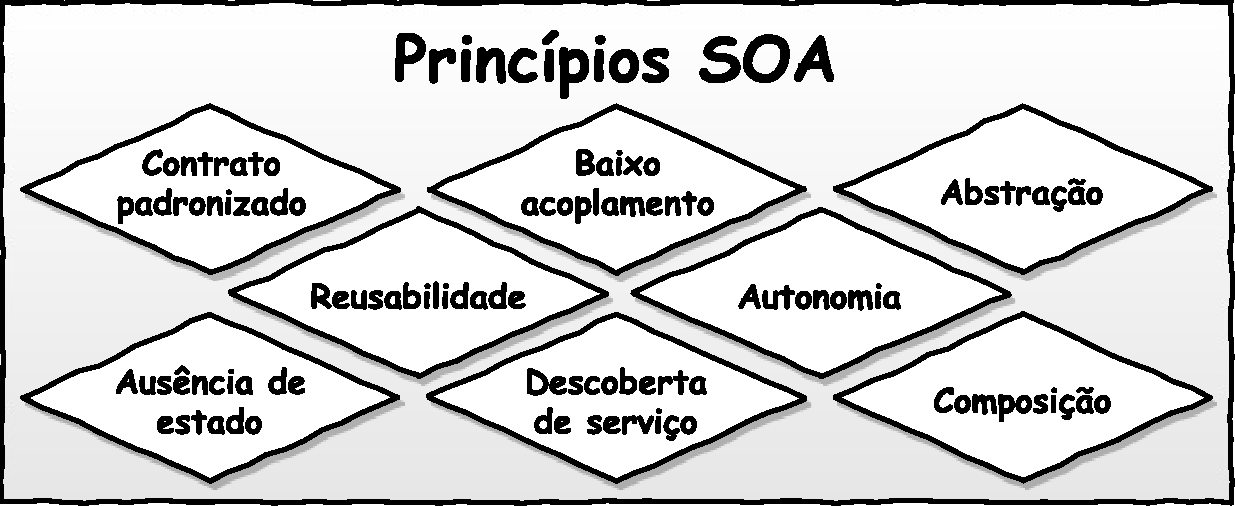
\includegraphics[width=100mm,trim = 0mm 0mm 0mm 
0mm,clip]{img/PrincipiosSOA.pdf}
\caption{Oito princípios da arquitetura orientada a serviços \cite{erl2009web}}
\label{Fig:PrincipiosSoa}
\end{figure}

\begin{description}
\item[Contrato padronizado] - \textbf{Serviços dentro de um mesmo inventário
estão em conformidade com os mesmos padrões de contrato de serviço}.
Os contratos de serviços são elementos fundamentais na arquitetura orientada a
serviço, pois é por meio deles que os serviços interagem uns com os outros e com
potenciais consumidores. Este princípio tem como foco principal o contrato de
serviço e seus requisitos. O padrão de projeto \CtFirst{} é uma
consequência direta deste princípio \cite{erl2009web}.

\item[Baixo acomplamento] - \textbf{Os contratos de serviços impõem aos
consumidores do serviço requisitos de baixo acoplamento e são, os próprios
contratos, desacoplados do seu ambiente}. 
Este princípio também possui forte relação com o contratos de serviço, pois a
forma como o contrato é projetado e posicionado na arquitetura é que gerará o
benefício do baixo acoplamento. O projeto deve garantir que o contrato
possua tão somente as informações necessárias para possibilitar a compreensão e
o consumo do serviço, bem como não possuir outras características que gerem
acoplamento.

São considerados negativos, e que devem ser evitados, os acoplamentos  
\begin{enumerate}[(a)] 
\item do contrato com as funcionalidades que ele suporta, agregando ao
contrato características específicas dos processos que o serviço atende;
\item do contrato com a sua implementação, invertendo a estratégia de conceber
primeiramente o contrato;
\item do contrato com a sua lógica interna, expondo aos consumidores
características que levem os consumidores a inadivertidamente aumentarem o
acoplamento;
\item do contrato com a tecnologia do serviço, causando impactos indesejáveis em
caso de substituição de tecnologia.
\end{enumerate}

Por outro lado, há um tipo de acoplamento positivo que é o que gera dependência
da lógica em relação ao contrato \cite{erl2009web}. Ou seja, idealmente a
implementação do serviço deve ser derivada do contrato, pondendo se ter inclusive a geração de código a
partir do contrato.


\item[Abstração] - \textbf{Os contratos de serviços devem conter apenas
informações essenciais e as informações sobre os serviços são limitadas àquelas
publicadas em seus contratos}. O contrato é a forma oficial a partir da qual o
consumidor do serviço faz seu projeto e tudo o que está além do contrato deve
ser desconhecido por ele. Por um lado este princípio busca a ocultação
controlada de informações. Por outro, visa a simplificação de informações do
contrato de modo a assegurar que apenas informações essenciais estão
disponíveis.


\item[Reusabilidade]- \textbf{Serviços contém e expressam lógica agnóstica e
podem ser disponibilizados como recursos reutilizáveis}. Este princípio
contribui para se entender o serviço como um produto e seu contrato com uma API
genérica para potenciais consumidores. Essa abordagem aplicada ao projeto dos
serviços leva a desenhá-lo com lógicas não dependentes de processos de negócio
específicos, de modo a torná-los reutilizáveis em vários processos.

\item[Autonomia]- \textbf{Serviços exercem um elevado nível de controle sobre
o seu ambiente em tempo de execução}. O controle do ambiente não está ligado a
dependência do serviço à sua plataforma em termos de projeto, mas sim ao aumento
da confiabilidade sobre a execução e redução da dependência dos recursos
sobre os quais não se tem controle.
O que se busca é a previsibilidade sobre o comportamento do serviço.

\item[Ausência de estado] - \textbf{Serviços reduzem o consumo de recursos
restringindo a gestão de estado das informações apenas a quando for necessário}.
Este princípio visa reduzir ou mesmo remover a sobrecarga gerada pelo
gerenciamento do estado de cada operação, aumentando a escalabilidade da
plataforma de arquitetura orientação a serviço como um todo. Na composição do
serviço, o serviço deve armazenar apenas os dados necessários para completar o
processamento, enquanto se aguarda o processamento do serviço acionado.

\item[Descoberta de serviço] - \textbf{Serviços devem conter metadados por meio
dos quais os serviços possam ser descobertos e interpretados}. Tornar cada
serviço de fácil descoberta e interpreção pelas equipes de projeto é o foco
deste princípio. Os próprios contratos de serviço devem ser projetados para
incorporar informações que auxiliem na sua descoberta.

\item[Composição] - \textbf{Serviços são participantes efetivos de composição,
independentemente do tamanho ou complexidade da composição}. O princípio da
composição faz com que os projetos de serviços sejam projetados para
possibilitar que eles se tornem participantes de composições. Deve-se levar em
conta, entretanto, os outros princípios no planejamento de uma nova composição,
considerando a complexidade das composições a serem formadas.

\end{description}
 

\subsection{Contract First}
\label{Contract-First}
\vspace{-6mm}

O princípio do baixo acoplamento tem por objetivo principal reduzir o
acoplamento entre o cliente e o fornecedor do serviço. Há vários tipos de
acoplamentos negativos, como citado na Subseção \ref{PrincipiosSOA}. Porém, um
acoplamento é considerado positivo e desejável: da implementação a partir do contrato. Ou seja, a lógica
do serviço deve corresponder ao que está especificado no contrato, permitindo
assim que o serviço seja reutilizado exclusivamente com conhecimento do
contrato.

Duas abordagens podem ser seguidas para se produzir esse efeito. A primeira é a
geração do contrato a partir da lógica implementada, conhecida como
\CdFirst{}. A outra propõe um sentido inverso, partindo-se do contrato
para a geração do código, chamada \CtFirst{}. A construção do serviço a
partir da modelagem do contrato, defendida na abordagem \CtFirst{}, é
recomendada para a arquitetura orientada a serviço \cite{erl2009web}.

Embora muitas vezes preferível pelo desenvolvedor, a desvantagem do uso
\CdFirst{} está no elevado impacto que alterações na implementação causam ao
contrato, fazendo com que os clientes dos serviços sejam também afetados.
Reduz-se a flexibilidade e extensibilidade, de modo que o reuso é prejudicado. Ainda,
eleva-se o risco de os serviços serem projetados para aplicações específicas e
não voltados para reuso e composição \cite{karthikeyancontract}.

A abordagem \CtFirst{} preocupa-se principalmente com a clareza, completude e
estabilidade do contrato para os clientes dos serviços. Toda a
estrutura da informação é definida sem a preocupação sobre restrições ou
características das implementações subjacentes. Do mesmo modo, as
capacidades são definidas para atenderem a funcionalidades a que se destinam,
porém com a preocupação em se promover estabilidade e reuso.

As principais vantagens do \CtFirst{} estão no baixo acoplamento do contrato em
relação a sua implementação, na possibilidade de reuso de esquemas de dados (XML
ou JSON Schema), na simplificação do versionamento e na facilidade de manutenção
\cite{karthikeyancontract}. A desvantagem está justamente na complexidade de
escrita do contrato. Porém, várias ferramentas já foram e vem sendo
desenvolvidas para facilitar essa tarefa.


\section{WEB SERVICES}
\vspace{-6mm}

\ws{} são aplicações modulares e autocontidas que podem ser publicadas,
localizadas a acessadas pela \textit{Web} \cite{alonso2004web}. A diferença
entre o \ws{} e a aplicação \textit{Web} propriamente dita é que o primeiro se
preocupa apenas com o dado gravado ou fornecido, deixando para o cliente a atribuição de apresentar a
informação \cite{serrano2014service}.

A necessidade das organizações de integrar suas soluções, seja
entre os sistemas internos ou entre esses e sistemas de outras empresas
\cite{rao2004survey}, não é recente. Essa é uma das principais motivações do uso
de \ws{}, por possibilitar que soluções construídas com tecnologias distintas
possam trocar informações por meio da \textit{Web}. Nesse contexto, as arquiteturas
orientadas a serviço fazem amplo uso de \ws{} como meio para disponibilização de serviços.

Há dois tipos de \ws{}: baseados em SOAP e baseados em REST. Os mais diversos
tipos de aplicações podem ser concebidas utilizando \wss{} SOAP ou REST,
situação também aplicável a serviços.
Originalmente os serviços utilizaram \ws{} SOAP, trafegando as informações em
uma mensagem codificada em um formato de troca de dados (XML), por meio do
protocolo SOAP (Seção \ref{secaoSOAP}). Entretanto, a adoção de \ws{} REST
(Seção \ref{secaoREST}) tem ganhado popularidade \cite{mumbaikar2013web}.

\subsection{SOAP (W3C) }
\label{secaoSOAP}
\vspace{-6mm}

SOAP -- \textit{Simple Object Access Protocol} -- é um protocolo padrão W3C que
provê uma definição de como trocar informações estruturadas, por meio de XML, entre
as partes de ambientes descentralizados ou distribuídos \cite{WSDLSite}. SOAP
é um protocolo mais antigo que REST, e foi desenvolvido para troca de informações
pela Internet se utilizando de protocolos como HTTP, SMTP, FTP, sendo o primeiro
o mais comumente utilizado.

Por ser anterior, SOAP é o padrão de \ws{} mais comumente utilizado pela
indústria.
Algumas pessoas chegam a tratar \ws{} apenas como SOAP e WSDL
\cite{serrano2014service}. SOAP atua como um envelope que transporta a mensagem
XML, e possui vastos padrões para transformar e proteger a mensagem e a
trasmissão. 


\subsubsection{Especificação de contratos}
\vspace{-6mm}

Os contratos em SOAP são especificados no padrão WSDL -- \textit{Web Services
Description Language} -- que define uma gramática XML para descrever os serviços
como uma coleção de \textit{endpoints} capazes de atuar na troca de mensagens.
As mensagens e operações são descritas abstratamente na primeira seção do
documento. Uma segunda seção, dita concreta, estabelece o protocolo de rede e o
formato das mensagens.

Muitas organizações preferem utilizar SOAP por ele dispor de mais mecanismos de
segurança e tratamento de erros \cite{serrano2014service}. Além disso, a tipagem
de dados é mais forte em SOAP que em REST \cite{mumbaikar2013web}, uma vez que
em SOAP se pode fazer uso de restrições e regras de validação providas pelo
padrão \textit{XML Schema} \cite{XMLSchema}.


\subsection{REST (Fielding)}
\label{secaoREST}
\vspace{-6mm}

O termo REST foi criado por Roy Fielding, em sua tese de doutorado
\cite{fielding2000architectural}, para descrever um modelo arquitetural
distribuído de sistemas hipermedia. Um \ws{} REST é baseado no conceito de
recurso (que é qualquer coisa que possua uma \textit{Uniform Resource
Identifier} -- URI) que pode ter zero ou mais representações
\cite{he2003service}.

O estilo arquitetural REST é cliente-servidor, em que o cliente envia uma
requisição por um determinado recurso ao servidor e este retorna uma resposta.
Tanto a requisição como a resposta ocorrem por meio da transferência de
representações de recursos \cite{mumbaikar2013web}, que podem ser de vários
formatos, como XML e JSON \cite{serrano2014service}. Toda troca de informações
ocorre por meio do protocolo HTTP, com uma semântica específica para cada
operação:

\begin{enumerate}
\item HTTP GET é usado para obter a representação de um recurso.
\item HTTP DELETE é usado para remover a representação de um recurso.
\item HTTP POST é usado para atualizar ou criar a representação de um recurso.
\item HTTP PUT é usado para criar a representação de um recurso.
\end{enumerate}

As transações são independentes entre si e com as transações anteriores, pois o
servidor não guarda qualquer informação de sessão do cliente. Todas as
informações de estado são trafegadas nas próprias requisições, de modo que as
respostas também são independentes. Essas características tornam os \wss{} REST
simples e leves \cite{mumbaikar2013web}.

O uso de REST tem se tornado popular por conta de sua flexibilidade e
performance em comparação com SOAP, que precisa envelopar suas informações em
um pacote XML \cite{mumbaikar2013web}, de armazenamento, transmissão e
processamento onerosos.

\subsubsection{Especificação de contratos}
\vspace{-6mm}

Ao contrário de SOAP, REST não dispõe de um padrão para especificação de
contratos. Essa carência, que no início não era considerada um problema, foi se
tornando uma necessidade cada vez mais evidente a medida em que se amplia o
conjunto de \wss{} implantados. Atualmente, existem algumas linguagens com o
propósito de documentar o contrato REST.

A linguagem mais popular atualmente é \textit{Swagger} cujo projeto se iniciou
por volta de 2010 para atender a necessidade de um projeto específico, sendo posteriormente
vendida para uma grande empresa. Em janeiro de 2016, \textit{Swagger} foi doada
para o \textit{Open API Iniciative (OAI)} e denominada de \textit{Open API
Specification}. O propósito da iniciativa é tornar \textit{Swagger} padrão para
especificação de APIs com independencia de fornecedor. Apoiam o projeto grandes
empresas como Google\textsuperscript{\textregistered},
Microsoft\textsuperscript{\textregistered} e
IBM\textsuperscript{\textregistered}.

WADL (\textit{Web Application Description Language}), uma especifição baseada em
XML semelhante ao WSDL, foi projetada e proposta pela \textit{Sun
Microsystems}\textsuperscript{\textregistered} e sua última versão submetida
ao W3C em 2009. Outra linguagem proposta é a RAML\cite{RAML} -- abreviação de
\textit{RESTful API Modeling Language} -- baseada em YAML e projetada pela
MuleSoft\textsuperscript{\textregistered}. Muitos projetos \textit{open source} adotam RAML.

Todas estas linguagens possuem suporte tanto para \CdFirst{} como para
\CtFirst{} \cite{wideberg2015restful}.



%\subsubsection{Outros padrões }
%\vspace{-6mm}
%\ldots

\section{DESIGN BY CONTRACT}
\label{Design-by-Contract}
\vspace{-6mm}

\designbycontract{} \cite{meyer1992applying} - DbC - é um conceito
oriundo da orientação a objetos, no qual consumidor e fornecedor firmam entre si garantias para
o uso de métodos ou classes. De um lado o consumidor deve garantir que, antes da
chamada a um método, algumas condições sejam por ele satisfeitas.
Do outro lado o fornecedor deve garantir, se respeitadas suas exigências,
o sucesso da execução.

O mecanismo que expressa essas condições são chamados de asserções
(\textit{assertions}, em inglês). As asserções que o consumidor deve respeitar
para fazer uso da rotina são chamadas de \textbf{precondições}. As asserções que
asseguram, de parte do fornecedor, as garantias ao consumidor, são denominadas
\textbf{pós-condições}.

DbC tem o objetivo de aumentar a robustez do sistema e tem na linguagem Eiffel
\cite{meyer1988eiffel} um de seus precursores. Para os mantenedores do Eiffel, DbC é
tão importante quanto classes, objetos, herança, etc. O uso de DbC na
concepção de sistemas é uma abordagem sistemática que produz sistemas com mais
corretude.

O conceito chave de \designbycontract{} é ver a relação entre a classe e
seus clientes como uma relação formal, que expressa os direitos e as
obrigações de cada parte \cite{meyer1997object}. Se, por um lado, o
cliente tem a obrigação de respeitar as condições impostas pelo fornecedor para fazer uso do módulo, por
outro, o fornecedor deve garantir que o retorno ocorra como esperado.

As precondições vinculam o cliente, no sentido de definir as condições que
o habilitam para acionar o recurso. Corresponde a uma obrigação para o cliente e
o benefício para o fornecedor \cite{meyer1997object} de que certos
pressupostos serão sempre respeitados nas chamadas à rotina.
As pós-condições vinculam o fornecedor, de modo a definir as condições para que o retorno ocorra.
Corresponde a uma obrigação para o fornecedor e o benefício para o cliente de
que certas propriedades serão respeitadas após a chamada à rotina.

De forma indireta, \designbycontract{} estimula um cuidado maior na análise das
condições necessárias para, de forma consistente, se ter o funcionamento correto
da relação de cooperação cliente-fornecedor.
Essas condições são expressas em cada contrato, o qual especifica as obrigações
a que cada parte está condicionada e, em contra-ponto, os benefícios garantidos.

Nesse contexto, o contrato é um veículo de comunicação, por meio do qual os
clientes tomam conhecimento das condições de uso, em especial das precondições.
É fundamental que as precondições estejam acessíveis para todos os clientes
para os quais as rotinas estão disponíveis, pois, sem que isso ocorra, o cliente
corre o risco de acionar a rotina fora de suas garantias de funcionamento. 

Segundo Bertrand Meyer \cite{meyer1997object}, \designbycontract{} é um
ferramental para análise, projeto, implementação e documentação, facilitando a
construção de \textit{softwares} cuja confiabilidade é embutida, no lugar de
buscar essa característica por meio de depuração. Meyer utiliza uma expressão de
Harlan D. Mills \cite{mills1975new} para afirmar que \designbycontract{} permite
construir programas corretos e saber que eles estão corretos.

Com o uso de \designbycontract{}, cada rotina é levada a realizar o trabalho
para o qual foi projetada e fazer isso bem: com corretude, eficiência e
genericamente suficiente para ser reusada. Por outro lado, especifica de forma
clara o que a rotina não trata. Esse paradigma é coerente, pois para que a
rotina realize seu trabalho bem, é esperado que se estabeleça bem as
circunstâncias de execução.

Outra característica da aplicação de \designbycontract{} é que o recurso tem sua
lógica concentrada em efetivamente cumprir com sua função principal, deixando
para as precondições o encargo de validar as entradas de dados. Essa abordagem
é o oposto à ideia de programação defensiva, pois vai de encontro à realização
de checagens redundantes. Se os contratos são precisos e explícitos, não há
necessidade de testes redundantes \cite{meyer1992applying}.

Todos esses aspectos são fundamentais para se possibilitar o reuso eficiente de
componentes, que é o pilar da orientação a objetos e se aplica de forma análoga
à orientação a serviços. Componentes reusáveis por várias aplicações devem ser
robustos pois as consequências de falhas ou comportamentos incorretos são muito
piores que as de aplicações que atendem a único propósito
\cite{meyer1992applying}.

Há de se registrar ainda que, em orientação a objetos, existe outro tipo de
asserção além das pré e pós-condições. Em vez de cuidar das propriedades de cada
rotina individualmente, elas expressam condições globais para todas as
instâncias de uma classe \cite{meyer1997object}. Essa categoria de
asserção é denominada invariante. Uma vez que em orientação a serviço se
preconiza a ausência de estado, o conceito de invariante não é explorado neste
trabalho, sem prejuízo da realização de estudo específico sobre o tema.



\subsection{Implementações de DbC}
\label{implementDbC}

\begin{description}
\item[Eiffel] - A linguagem Eiffel foi desenvolvida em meados dos anos 80 por
Bertrand Meyer \cite{meyer1988eiffel} com o objetivo de criar ferramentas que
garantissem mais qualidade aos \textit{softwares}. A ênfase do projeto de
Eiffel foi promover reusabilidade, extensibilidade e compatibilidade.
Características que só fazem sentido se os programas forem corretos e
robustos.

Foi essa preocupação que incorporou à linguagem Eiffel o conceito de contratos.
A partir desse estilo de projeto se criou a noção de \designbycontract{},
concretizada na linguagem por meio das precondições, pós-condições e invariantes
\cite{meyer1988eiffel}. Esta abordagem influenciou outras linguagem de programação orientadas a objeto.

A Figura \ref{lst:exemploEiffel} apresenta um exemplo de especificação de pré e
pós-condição na linguagem Eiffel.

\vspace{6mm}

\begin{figure}[h]
\begin{small}
\lstinputlisting[language=Eiffel,firstnumber=1]{trechos_codigo/exemploEiffel.tex}
\vspace{-.5cm}
\end{small}
\caption{Exemplo de pré e pós-condições em Eiffel}
\label{lst:exemploEiffel}
\end{figure}


\item[JML] - \textit{Java Modeling Language} é uma extensão da linguagem Java
para suporte a especificação comportamental de interfaces, ou seja, controlar o
comportamento de classes em tempo de execução. Para realizar essa função, JML
possui amplo suporte a \designbycontract{}. As asserções (precondição,
pós-condição e invariantes) são incluídas no código Java na forma de comentários
(//@ ou /*@\ldots@*/).

JML combina a praticidade de \designbycontract{} de linguagens como Eiffel com a
expressividade e formalismo de linguagens de especificação orientadas a modelo
\cite{leavens2006design}. 

A Figura \ref{lst:exemploJML} apresenta um exemplo de especificação de pré e
pós-condição na linguagem de extensão JML.

\begin{figure}[h]
\begin{small}
\lstinputlisting[language=JML,firstnumber=1]{trechos_codigo/exemploJML.tex}
\vspace{-.5cm}
\end{small}
\caption{Exemplo de pré e pós-condições em JML}
\label{lst:exemploJML}
\end{figure} 
 
\vspace{8mm}

\item[Spec\#] - é uma extensão da linguagem C\#, à qual agrega o suporte para
distinguir referência de objetos nulos de referência a objetos possivelmente não
nulos, especificações de pré e pós-condições e um método para gerenciar
exceções entre outros recursos \cite{barnett2004spec}.

A Figura \ref{lst:exemploSpec} apresenta um exemplo de especificação de pré e
pós-condição na linguagem Spec\#.

\vspace{6mm}

\begin{figure}[h]
\begin{small}
\lstinputlisting[language=SpecSharp,firstnumber=1]{trechos_codigo/exemploSpecSharp.tex}
\vspace{-.5cm}
\end{small}
\caption{Exemplo de pré e pós-condições em Spec\#}
\label{lst:exemploSpec}
\end{figure}

\vspace{8mm}

\item [Code Contract] - é uma maneira mais moderna que Spec\# para utilização de
construções de DbC no \textit{framework} .Net. \textit{Code Contract} inclui
classes para registrar as restrições (pré, pós-condições e invariantes) ao
código C\# e um analisador estático para análise em tempo de compilação e
execução \cite{codecontractSite}. 

O uso de \textit{Code Contract} também permite a geração de documentação da API
com as informações do contrato. Estão disponíveis ainda ferramentas para geração
de testes unitários para verificação das pré condições. A Figura \ref{lst:exemploCodeContract}
apresenta um exemplo de especificação de pré e pós-condição em \textit{Code
Contract}.

\vspace{6mm}

\begin{figure}[h]
\begin{small}
\lstinputlisting[language=CodeContract,firstnumber=1]{trechos_codigo/exemploCodeContract.tex}
\vspace{-.5cm}
\end{small}
\caption{Exemplo de pré e pós-condições em Code Contract}
\label{lst:exemploCodeContract}
\end{figure}

\end{description}





 


% 3. NeoIDL - Objetivos / Resultados / Avaliação empírica / Extensão da
% Linguagem  / Estudo de caso
\chapter{NEOIDL: LINGUAGEM PARA ESPECIFICAÇÃO DE CONTRATOS REST	}
\vspace{-6mm}


\section{APRESENTAÇÃO}
\label{apresentacaoNeoIDL}

A \neoidl{} é uma linguagem específica de domínio (\textit{Domain Specific
Language - DSL}) elaborada com o objetivo de possibilitar, em um processo
simples, a elaboração de contratos para serviços REST. Em seu projeto, 
foram considerados os requisitos de concisão, facilidade de compreensão humana,
extensibilidade e suporte à herança simples dos tipos de dados definidos pelo
usuário.

Além de ser uma linguagem, a \neoidl{} é também um \textit{framework} de geração
de código que permite, a partir de contratos especificados na própria
linguagem, a produção da implementação da estrutura do serviço. Os serviços
podem ser construídos em várias linguagens e tecnologias, por meio
de \textit{pluggins} da \neoidl{}.

As próximas subseções apresentam o histórico da \neoidl{}, exemplificam sua
sintaxe e descrevem sucintamente seu \textit{framework} de geração de código.


\subsection{Histórico e motivação}
\label{histMotivNeoIDL}
\vspace{-6mm}

A \neoidl{} surgiu no contexto de um acordo de colaboração entre a Universidade
de Brasília e o Exército Brasileiro. O projeto do exército caracterizava-se
pelos requisitos de modularidade -- com a lógica distribuída inclusive
geograficamente -- e de execução em plataformas diversificadas. Diante dessa
necessidade, o Exército desenvolveu um \textit{framework} proprietário,
voltado para arquitetura orientada a serviço e com suporte
a implantação de serviços REST em vários linguagens, denominado \neocortex{}.

A particularidade do \neocortex{} de se utilizar serviços implementados em
vários linguagens motivou o desenvolvimento um programa gerador de serviços
poliglotas -- que produz código de várias linguagens de programação -- a partir da
descrição do contrato do serviço. A \neoidl{} foi concebida para atender a essa
finalidade. A primeira decisão de projeto da \neoidl{} foi a linguagem para se
especificar o contrato de serviço.

Porém, as linguagens de programação disponíveis para especificação de
contratos REST, como Swagger\cite{swaggerSite}, WADL\cite{hadley2006web} e
RAML\cite{RAML}, possuiam (e ainda possuem) limitações importantes para a
abordagem desejada, qual seja elaborar primeiramente o contrato e, a
partir dele, gerar a implementação do serviço. Todas essas linguagens utilizam
notações de propósito geral (XML\cite{XML}, JSON\cite{JSon}, YAML\cite{YAML}),
tornando os contratos extensos e de difícil compreensão humana. Além disso,
elas não possuem mecanismos semânticos de extensibilidade e modularidade.

Partiu-se então para a criação uma nova linguagem, com sintaxe
inspirada em linguagens mais claras e concisas -- como emph{CORBA
IDL}\texttrademark \cite{corba} e \emph{Apache
Thrift}\texttrademark\cite{thrift} --, e que permitisse ainda a declaração de
tipos de dados definidos pelo usuário e extensibilidade. Ambas, \emph{CORBA} e
\emph{Apache Thrift}, possuem limitações nesses últimos aspectos. A sintaxe e as
características da linguagem \neoidl{} são brevemente discutidas na subseção
\ref{linguagemNeoIDL}.

Em relação à geração de código, para se viabilizar a geração poliglota de
código, a \neoidl{} foi projetada para possui uma arquitetura modular, de modo que novas linguagens ou características de implementaçao
pudessem ser incorporadas por meio de \textit{plugins} da \neoidl{}. Assim, é
possível desenvolver um novo \textit{plugin} para geração de serviços em outras
linguagens, por exemplo PHP, sem alterar qualquer outro componente do \framework,
conforme apresentado na subseção \ref{frameNeoIDL}.

A primeira versão da \neoidl{}, ponto de onde partiu este trabalho de mestrado,
dava suporte à geração de código em Java, Python e Swagger com as
características necessárias para execução no \neocortex{}. Nessa versão, foram
desenvolvidos para o Exército Brasileiro nove serviços do domínio de Comando e
Controle \cite{david:commandControl}, os quais compreenderam aproximadamente
cinquenta módulos\footnote{O conjunto de documentos
utilizados para descrever contratos na \neoidl{} são denominados
\texttt{módulos}.} e geração de três mil linhas de código Python a partir
da especificação dos contrato em \neoidl{}. Alguns outros serviços foram
ainda implementados em Java.



\subsection{Linguagem}
\label{linguagemNeoIDL}
\vspace{-6mm}

A linguagem \neoidl{} simplifica a especificação de contratos REST pois possui
uma sintaxe concisa, própria de linguagens de especificação de interfaces
(\emph{interface description languages}). Ademais, a \neoidl{} provê mecanismos de
modularização e herança, de forma que os contratos possam ser separados em
módulos, facilitando a herança e manutenção dos
contratos. 

Para demonstrar como os módulos são estruturados na
\neoidl{}, a seguir são apresentados alguns trechos de um serviço hipotético
de envio de mensagens. Na primeira parte, um módulo faz uma definição de tipo
de dado; em seguida, um segundo módulo, voltado para especificação do serviço em
si, importa as definições do primeiro para então declarar as operações do
serviço. Por fim, ao módulo de serviço é acrescentada uma anotação como
forma de extender as características da operação.

\vspace{6mm}

\begin{figure}[h]
\begin{small}
\lstinputlisting[language=NeoIDL,firstnumber=1]{trechos_codigo/mensagemData.tex}
\vspace{-.5cm}
\end{small} 
\caption{Tipos de dados definidos na \neoidl}
\label{lst:messagedata-neo}
\end{figure}

O trecho ilustrado na figura \ref{lst:messagedata-neo} faz a definição de dois
tipos de dados. \emph{MessageType}, declarado no linha 2, é uma estrutura
simples do tipo enumeração. No exemplo, \emph{MessageType} pode ter os valores
\emph{Received} e \emph{Send}.
O outro tipo é \emph{Message}, declarado entre as linhas 4 e 11,
composto de seis atributos (\emph{id, from, to, subject, content} e
\emph{type}).
O atributo \emph{type} de \emph{Message} é do tipo \emph{MessageType} recém declarado.

Na \neoidl{}, é utilizada a abordagem \emph{convenção sobre configuração}, de
modo que todos os atributos declarados são obrigatórios, a menos que
seja explicitamente declarado diferente. O atributo \emph{subject} do tipo
\emph{Message} é um exemplo de atributo opcional (\texttt{<Type> <Ident> = 0;}).

Definido o tipo de dado, o módulo seguinte (figura \ref{lst:sentmessage-neo})
, na linha proposta pela \neoidl{} para suporte a herança
e reuso, importa o conjunto de definições de \emph{MessageData} e declara o
serviço \emph{sendbox} (linha 4). Esse serviço possui duas capacidades:
\emph{sendMessage} e \emph{listMessages}.
A capacidade \emph{sendMessage} (linha 6) utiliza a operação \method{post} para
submeter uma mensagem (tipo \emph{Message}). A capacidade \emph{listMessages}
(linha 7) tem a finalidade de listar as mensagens com um determinado sequecial,
por meio da operação \method{get}.

A instrução \emph{path} (linha 5) completa a especificação do serviço, indicando
o caminho (URI) onde as operações serão disponibilizadas. Esse atribuito é importante para se definir
como as requisições serão roteadas entre os serviços.

\vspace{6mm}

\begin{figure}[htb]
\begin{small}
\lstinputlisting[language=NeoIDL,firstnumber=1]{trechos_codigo/mensagem.tex}
\end{small}
\caption{Sent message service specification in \neoidl}
\label{lst:sentmessage-neo}
\end{figure}

Seguindo a filosofia de \emph{conversão sobre configuração}, a \neoidl{} assume
que os argumentos das operações do tipos \method{POST} e \method{PUT} são
enviadas no corpo da requisição. Nas operações dos tipos \method{GET} e
\method{DELETE}, por outro lado, presume-se que os agumentos estão contidos no \emph{path} da requisição ou ainda
como \textit{query string}.

A especificação dos contratos na \neoidl{} pode ser enriquecida de forma simples
com o uso de anotações, pois elas possibilitam extender a semântica
de uma especificação sem que seja necessário alterar a sintaxe da
linguagem \neoidl{}. Essa versatilidade das anotações é bastante útil, pois a
alteração da sintaxe da própria \neoidl{} não é um esfoço trivial, por demandar
a compatibilização de todos os \textit{plugins} já construídos.

O módulo apresentado na figura \ref{lst:annotationNeoIDL} contém, além das
informações contidas no módulo da figura \ref{lst:sentmessage-neo}, uma anotação
denominada \emph{Security Policy} (linhas 4 a 6) que é aplicada ao serviço
\emph{sentbox}.
A declaração da anotação é feita ao final do módulo (linhas 14 a 18).

\vspace{6mm}
 
\begin{figure}[htb]
\begin{small}
\lstinputlisting[language=NeoIDL,firstnumber=1]{trechos_codigo/messageSendAnnotation.tex}
\vspace{-.5cm}
\end{small}
\caption{Especificação de anotação na \neoidl{}}
\label{lst:annotationNeoIDL}
\end{figure}

Além de serem aplicáveis a \texttt{resources}, as anotações também podem ser
utilizadas em outros construtores da linguagem: \texttt{module},
\texttt{enum}, \texttt{entity}. Qualquer anotação na \neoidl{} possui a mesma estrutura: um
nome, um elemento alvo e uma lista propriedades. Todas estas informações ficam
disponíveis para utilização pelos \textit{plugins}.

\begin{figure*}[h]
\begin{center}
\includegraphics[scale=0.55,trim=0cm 1.5cm 0cm
0cm]{img/EstruturaModuloNeoIDL.png}  
\end{center}
\caption{Módulo \neoidl{}}
\label{fig:moduloNeoIDL}
\end{figure*}


A estrutura de um módulo \neoidl{}, como pôde ser verificado nos exemplos
acima e ilustrada na Figura \ref{fig:moduloNeoIDL}, é composta pelas seguintes
seções: assinatura do módulo, seção de importação, enumerações e estruturas,
serviços e anotações. O apêndice \ref{apend:estruturaLexicaNeoIDL} apresenta a
estrutura sintática e léxica da \neoidl{} antes de terem sido incorporadas as construções
relativas a \designbycontract{}.



\subsection{\textit{Framework}}
\label{frameNeoIDL}
\vspace{-6mm}

A parte da \neoidl{} responsável pela geração de código de
serviço para as várias linguagens é denominado \framework{} \neoidl{}. O
\framework{} \neoidl{} possui suas partes: o núcleo e os \textit{plugins},
conforme ilustrado na figura \ref{fig:programGenerator}.
O núcleo é composto de módulos responsáveis (a) por fazer o \textit{parse}\footnote{O \textit{parser} da \neoidl{}
foi construído utilizando \bnfc{} \cite{ranta-bnfc:2012} com a linguagem de
programação funcional Haskell.}
do contrato escrito em \neoidl{}, (b) por processar a sintaxe da linguagem \neoidl{} e (c) pelo gerenciamento dos \textit{plugins}.

Fora do núcleo da \neoidl{} ficam os \textit{plugins}, responsáveis,
cada um, por gerar código para as linguagens de destino. Assim, para se
possibilitar a geração de código para uma nova linguagem ou segundo uma nova arquitetura, um
novo \textit{plugin} deve ser desenvolvido. A primeira versão da \neoidl{}
possuia \textit{plugins} para Python, Java e Swagger.

\begin{figure*}[h]
\begin{center}
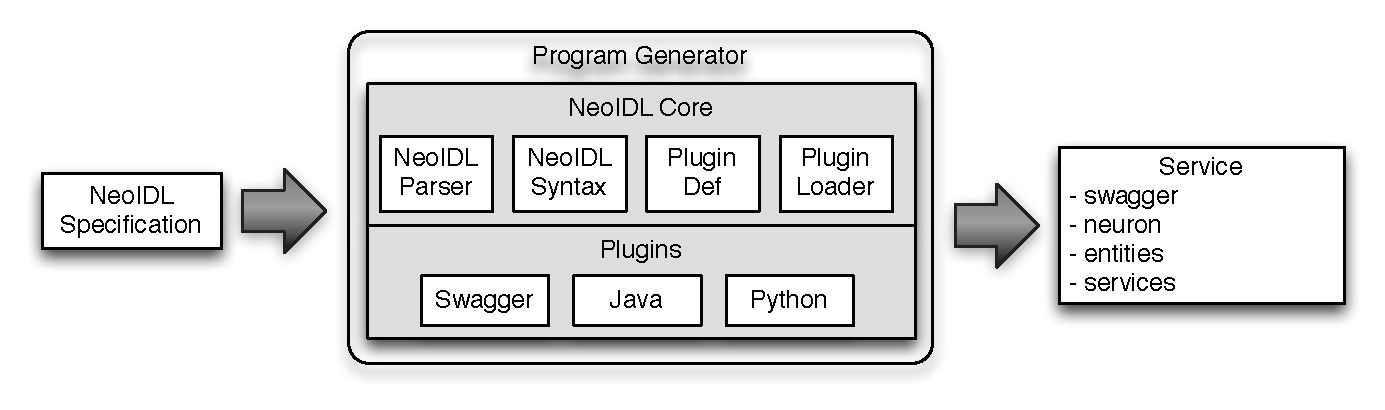
\includegraphics[scale=0.55,trim=0cm 1.5cm 0cm 0cm]{img/programgenerator.pdf}
\vspace{-.5cm}
\end{center}
\caption{Gerador de código da \neoidl{}}
\label{fig:programGenerator}
\end{figure*}

As próximas subseções resumem o funcionamento de
dois módulos onde estão contidas os principais trechos da lógica implementada na \neoidl{}: O
\textit{PluginDef} e \textit{PluginLoader}. Mais detalhes podem ser obtidos na
publicação \textit{NeoIDL: A Domain Specific Language for Specifying REST
Contracts Detailed Design and Extended Evaluation} \cite{lima2015neoidl}.
 

\subsubsection{Componente PluginDef}{\label{sec:plugindef}}

O módulo \texttt{PluginDef} estabelece as definições de regras de projeto
(\textit{Design Rules}) obrigatórias para o desenvolvimento de
\textit{plugins}, padronizando-os. De acordo com as regras de projeto, cada
\textit{plugin} precisa declarar uma instância do tipo \emph{Plugin} e implementar uma função de
transformação de acordo com a assinatura definida.

Além disso, cada instância de  
\texttt{Plugin} precisa ter o nome do \texttt{plugin} de forma que o
componenente \texttt{PluginLoader} (subseção \ref{compPluginLoader}) possa obter
os dados necessários para o seu processamento.
Resumidamente, a execução de um \textit{plugin} consiste em aplicar sua função
de transformação a um módulo \neoidl{} e produzir uma lista de
arquivos de código fonte. 


\subsubsection{Componente PluginLoader}
\label{compPluginLoader}

O carregamento e validação dos \textit{plugins} são competências do componente
\texttt{PluginLoader}. Se todas as regras de definição do \textit{plugin}
tiverem sido atendidas, o \textit{plugin} é carregado e estará pronto para ser
 acionado. Caso contrário, algumas exceções podem ocorrer, como, por exemplo, não haver definição de
nenhum \textit{plugin} no arquivo:

\begin{tabbing}\tt
~\char36{}\char46{}\char47{}neoIDL\\
\tt ~neoIDL\char58{}~panic\char33{}~\char40{}the~\char39{}impossible\char39{}~happened\char41{}\\
\tt ~~\char40{}GHC~version~7\char46{}6\char46{}3~for~x86\char95{}64\char45{}darwin\char41{}\char58{}\\
\tt ~~~~Not~in~scope\char58{}~\char96{}Plugins\char46{}Python\char46{}plugin\char39{}
\end{tabbing}

Ou ainda em razão de o \textit{plugin} não ser uma instância do tipo
\texttt{Plugin}:

\begin{tabbing}\tt
~\char36{}\char46{}\char47{}neoIDL\\
\tt ~neoIDL\char58{}~panic\char33{}~\char40{}the~\char39{}impossible\char39{}~happened\char41{}\\
\tt ~\char40{}GHC~version~7\char46{}6\char46{}3~for~x86\char95{}64\char45{}darwin\char41{}\char58{}\\
\tt ~~Couldn\char39{}t~match~expected~type~\char96{}Plugin\char39{}\\
\tt ~~~with~actual~type~\char96{}\char91{}GHC\char46{}Types\char46{}Char\char93{}\char39{}
\end{tabbing}


\section{AVALIAÇÃO EMPÍRICA}
\vspace{-6mm}

A primeira versão da \neoidl{} foi submetida a um estudo empírico de sua expressividade 
e reuso em um contexto real. As próximas subseções apresentam 
o resultado da análise comparativa da representação de 44 (quarenta e quatro)
contratos escritos em Swagger em relação à mesma especificação em \neoidl{}.

Esse estudo é uma das contribuições deste trabalho de mestrado e foi publicado
no periódico IJSeke \cite{lima2015neoidl}.

\subsection{Expressividade}
\label{estudoExpressividadeNeoIDL}
\vspace{-6mm}

A \neoidl{} é uma DSL, conforme apresentado na seção \ref{apresentacaoNeoIDL},
e como tal se destina a atender a um propósito específico, nem mais, nem menos
\cite{hudak1998modular}. A \neoidl{} foi projetada para permitir a
especificação de contratos de serviços REST de forma mais expressiva e concisa,
facilitando-se a escrita e leitura por humanos (mais detalhes na subseção
\ref{histMotivNeoIDL}).

Programas escritos em DSLs costumam ser mais fáceis de escrever e,
consequentemente, mais fáceis de se manter comparavelmente a programas escritos
em linguagens de propósito geral \cite{hudak1998modular}. Isso se deve
justamente ao fato de a DSL tratar apenas um conjunto reduzido de situações e
problemas, fazendo com ela seja, muitas vezes, mais acessível ao público geral
\cite{taha2008domain}.

A expressividade é um dos principais critérios para se escolher uma
linguagem. Entretanto a linguagem que não expressa todas as situações
necessárias ao seu contexto de uso, por óbvio, não pode ser usada
\cite{mackinlay1985expressiveness}. Nesse sentido, o primeiro teste a que a
\neoidl{} foi submetido constituiu-se na produção de contratos e serviços reais
no início do projeto com o Exército Brasileiro (vide subseção \ref{histMotivNeoIDL}).

Assim, tendo a \neoidl{} demonstrado sua capacidade de representar contratos
REST reais, foi realizada uma segunda análise: quão expressiva seria a
\neoidl{} em comparação com outra linguagem com o mesmo objetivo. Foi escolhida
Swagger \cite{swaggerSite}, uma linguagem de especificação de contratos REST
cujo uso tem crescido pela indústria.
Em Swagger, os contratos são escritos em JSON\cite{JSon} ou YAML\cite{YAML},
ambos com uma estrutura geral de chave-valor.

Sendo a facilidade de compreensão e manipulação por humanos um dos pilares
de desenvolvimento da \neoidl{}, foi adotada a estratégia de comparar a
expressividade em termos de quantidade de linhas de código (SLOC - do inglês
\textit{Source Lines of Code}), uma vez que muitas linhas significam maior
esforço para escrita, sobretudo na abordagem \CtFirst{}.

Com este propósito, foi obtido um conjunto de 44 contratos do Exército
Brasileiro especificados em Swagger. A primeira etapa foi reescrever esses
contratos em \neoidl{} e então comparar a quantidade de linhas de código
produzida com a quantidade de linhas de código dos contratos originais.

Para a
transcrição dos contratos, em razão da \neoidl{} não possuir recursos para
transcrição bidirecional de Swagger para \neoidl{}, foi desenvolvido
e utilizado um \textit{script} na linguagem \textit{Perl}, 
o qual consta do Apêndice desta dissertação
(Apêndice \ref{scriptSwagger2NeoIDL}).

Os quarenta e quatro contratos em Swagger contabilizaram 13.921 linhas de
especificação. Os mesmos contratos especificados em \neoidl{} somaram 5.140
linhas de especificação, correspondendo a uma redução média de 63\%. Assim, para
cada 10 linhas de especificação em Swagger são requeridas 4 linhas de
especificação \neoidl{}. Nessa análise foram consideradas linhas físicas de
código, ignorando-se linhas em branco ou compostas apenas de delimitadores.

A proporção de redução não se deu de forma igual em todos os contratos. Por
exemplo, o contrato de um determinado serviço\footnote{Os nomes reais dos
contratos foram omitidos em razão de acordo de confidencialidade.} requereu 367
linhas na especificação Swagger e 112 linhas na especificação \neoidl{} --
redução da ordem de 69\%.
Em contraponto, outro serviço especificado em Swagger possuia 81 linhas e o
correspondente em \neoidl{} 42 linhas -- redução de linhas de código pouco inferior a 50\%.

Estatisticamente, o tamanho original dos contratos tem apenas uma pequena
influência na expressividade avaliada. Dessa forma, não é possível assumir que
contratos Swagger maiores terão um correspondente proporcionalmente menor em
\neoidl{}.
Outros atributos como documentação mais descritiva, quantidade de entidades e o
número de capacidades de cada serviço também não possuem correlação com redução
de linha de código maior ou menor após o processo de tranformação para
\neoidl{}.

A tabela \ref{tab:size-corr} apresenta a correlação entre a
melhoria na expressividade observada (medida como percentual de redução após a
transformação da especificação Swagger em especificação \neoidl{}) e algumas
métricas relacionadas ao tamanho da especificação original em Swagger. Na
Correlação Pearson, um \emph{p-value} igual a 1 significa correlação
positiva perfeita. \emph{p-value} igual a -1, significa correlação negativa
perfeita, enquanto \emph{p-value} igual a zero indica que as medidas não possuem
correlação linear.

% 
% 
% Table~\ref{tab:size-corr} presents the correlation between the improvement of
% expressiveness (measured as the percentage of reduction obtained after
% transforming Swagger specifications into \neoidl{} specifications) and some
% metrics related to the size of the original Swagger specifications.

\begin{table}[htb]
\caption{Correlação da melhoria de expressividade com o tamanho da especificação
em Swagger}
\begin{center}
\begin{tabular}{lrr} 
\toprule
Métrica & Correlação Pearson's & \emph{p-value} \\ \hline \hline 
LOC da especificação Swagger & 0.19 &  0.20 \\ 
Número de serviços & 0.14 & 0.35 \\ 
Numero de capacidades & 0.14 & 0.34 \\
Número de entidades & 0.20 & 0.18 \\ \bottomrule 
\end{tabular} 
\end{center}
\label{tab:size-corr}
\end{table}





\subsection{Potencial de reuso}

De forma similar à \neoidl{}, Swagger também possui recursos para reuso de
estruturas, por meio de referências (marcação \$ref). Entretanto, esse recurso
praticamente não foi explorado no conjunto de contratos analisados, o que
ocasinou na duplicação da declaração de estruturas entre os diferentes arquivos
de especificação Swagger. Isso se deve, provavelmente, ao modo não intuitivo de
se fazer referência em Swagger (baseado na referência a outro arquivo JSON) e à
dificuldade de se identificar que uma determinada entidade foi declarada em
outro contrato.

No conjunto dos 44 contratos Swagger analisados foram identificadas 40 entidades
especificadas em pelo menos dois contratos. Uma entidade específica, de
identificação da posição geográfica, muito utilizada no domínio de Comando e Controle, aparece
declarada 12 vezes em contratos distintos.


% 4. Análise da aceitação - Método / GQM / Resultados
\chapter{CONTRATOS REST COM DESIGN-BY-CONTRACT}


\section{PROPOSTA: SERVIÇOS COM DESIGN-BY-CONTRACT}
\label{PropostaServicoDbC}
\vspace{-6mm}

Os benefícios esperados pela adoção da arquitetura orientada a serviços
somente serão auferidos com a concepção adequada de cada serviço. 
Por essa razão, é necessário planejar o projeto dos serviços criteriosamente
antes de lançar mão do desenvolvimento, com preocupação especial em garantir
um nível aceitável de estabilidade aos consumidores de cada serviço.
Nessa etapa do projeto de desenho da solução, a especificação do contrato do
serviço (Web API) exerce uma função fundamental. 

Na sociedade civil, contratos são meios de se formalizar acordo entre partes a
fim de definir os direitos e deveres de cada parte e buscar atingir o
objetivo esperado dentro de determinadas regras. Cada parte espera que as outras
cumpram com suas obrigações.
Por outro lado, sabe-se que o descumprimeto das obrigações costuma implicar de
penalizações até o desfazimento do contrato. 

Contratos entre serviços Web seguem em uma linha análoga. O desenho das
capacidades (operações) e dos dados das mensagens correspondem aos
termos do contrato no sentido do que o consumidor deve esperar do serviço
provedor. Porém identificou-se, após ampla pesquisa realizada sobre o tema, que
as linguagens disponíves para especificação de contratos atingem apenas esse
nível de garantias. No contexto de webservices em REST, conforme descrito na
seção \ref{secaoREST}, há ainda a ausência de padrão para especificação
contratos.

A proposta deste trabalho é extender os níveis de garantias, de modo a promover
um patamar adicional com obrigações mutuas entre os serviços (consumidor e
provedor). Isso se dá para adoção do conceito de \designbycontract{} (debatido
na seção \ref{Design-by-Contract}) em que a execução da
capacidade do serviço garantirá a execução, desde que satisfeitas as condições
prévias. As próximas subseções detalham o modo de operação dos serviços com as
construções de \designbycontract{}.

\vspace{-6mm}

\subsection{Modelo de operação}
\vspace{-6mm}

As garantias para execução dos serviços são estabelecidas em duas etapas: pré e
póscondições. Nas precondições o provedor do serviço estabelece os requisitos
para que o serviço possa ser executado pelo cliente. A etapa de pós-condições
tem o papel de validar se a mensagem de retorno do serviço possui os resultados
esperados.

O diagrama da Figura \ref{FigServiceDbC} descreve como ocorre a operação das
pré e pós-condições. O processo se inicia com a chamada à capacidade do serviço e a
identificação da existência de uma precondição. Caso tenham sido estabelecidas 
precondições, essas são avaliadas. Caso alguma delas não tenham sido
satisfeitas, o serviço principal não é processado e o provedor do serviço
retornar o código de falha definido no contrato correspondente.


\begin{figure}[!htb]
\centering
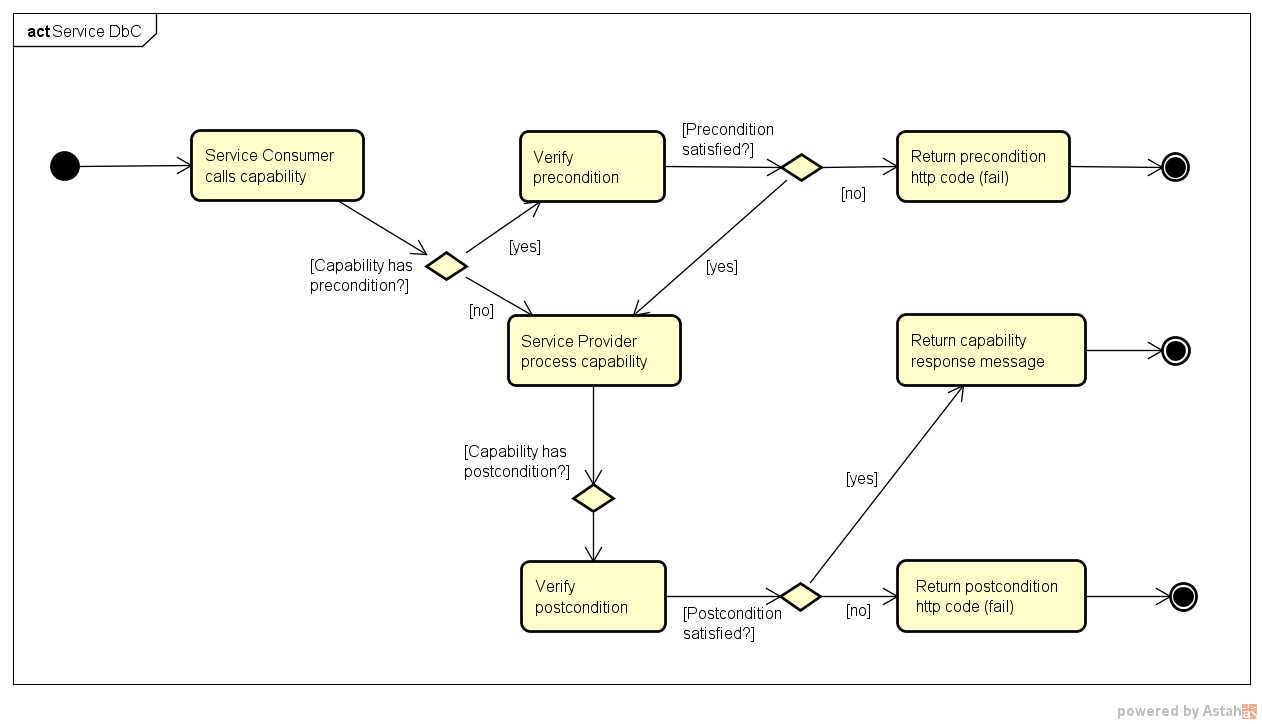
\includegraphics[width=\textwidth,trim = 0mm 5mm 0mm 0mm,clip]{ServiceDbC.png}
\caption{Digrama de atividades com verificação de pré e pós condições}
\label{FigServiceDbC}
\end{figure}

Caso tenham sido definidas pós-condições, essas são acionadas após o
processamento da capacidade, porém antes do retorno ao consumidor do serviço.
Assim, conforme Figura \ref{FigServiceDbC}, visando não entregar ao cliente uma
mensagem ou situação incoerente, as pós-condições são validadas. Caso todas as
pós-condições tenham sido satisfeitas, a mensagem de retorno é encaminhada ao
cliente. Caso contrário, será retornado o código de falha definido para a
pós-condição violada.

\subsubsection{Observação sobre invariantes}
\vspace{-6mm}

Em \designbycontract{}, além dos conceitos de pré e pós-condições,
há também a ideia de invariantes\cite{meyer1997object}. Quando aplicadas a uma classe na
orientação a objetos, as invariantes estabelecem restrições sobre o estado
armazenado nos objetos instanciados dessa classe. No contexto de orientação a
serviços, tem-se por princípio a ausência de estados dos serviços, descrito na
seção \ref{PrincipiosSOA}. Por essa razão, no estudo sobre a incorporação de
\designbycontract{} em contratos de serviços, as invariantes não foram
consideradas.


\subsection{Verificação das precondições}
\vspace{-6mm}

As precondições podem ser do tipo baseado nos parâmetros da requisição ou do
tipo baseado na chamada a outro serviço. Denomina-se, no contexto desta
dissertação, de básica a precondição baseada apenas nos parâmetros da
requisição (atributos da chamada ao serviço). Essa validação é direta,
comparando os valores passados com os valores admitidos. 

No caso das precondições baseadas em serviços, é realizada chamada a outro
serviço para verificar se uma determinada condição é satisfeita. Este modo de
funcionamento, que se assemelha a uma composição de serviço, é mais versátil, pois permite
validações de condições complexas sem que a lógica associada seja conhecida pelo
cliente. Assim, os contratos que estabelecem esse tipo de
precondição se mantem simples.

A Figura \ref{FigServicePrecondition} detalha as etapas de verificação de cada
precondição. Nota-se que a saída para as situações de desatendimento às
precondições, independentemente do tipo, é o mesmo. O objetivo desta abordagem
é simplificar o tratametno de exceção no consumidor.

\begin{figure}[!htb]
\centering
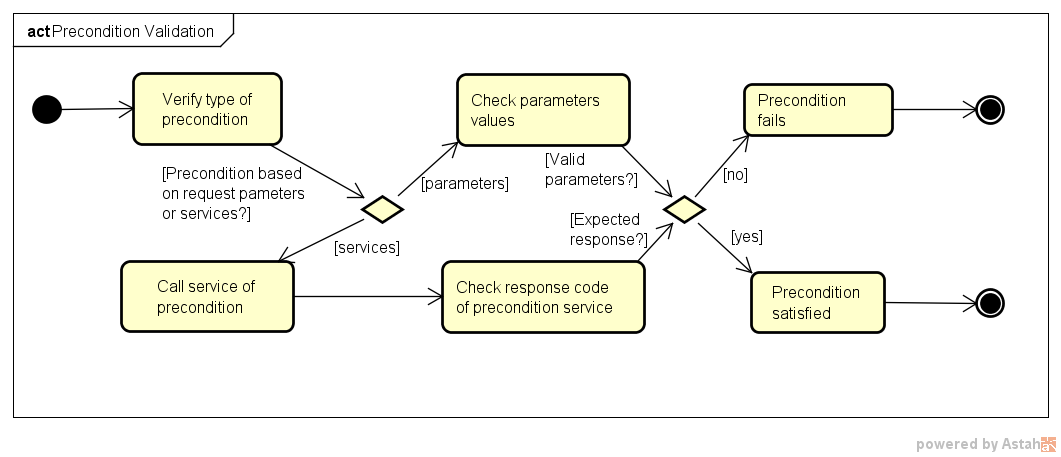
\includegraphics[width=\textwidth,trim = 0mm 5mm 0mm 0mm,clip]{PreconditionValidation.png}
\caption{Diagrama de atividades do processamento da precondição}
\label{FigServicePrecondition}
\end{figure}


\subsection{Verificação das pós-condições}
\vspace{-6mm}

\begin{figure}[!htb]
\centering
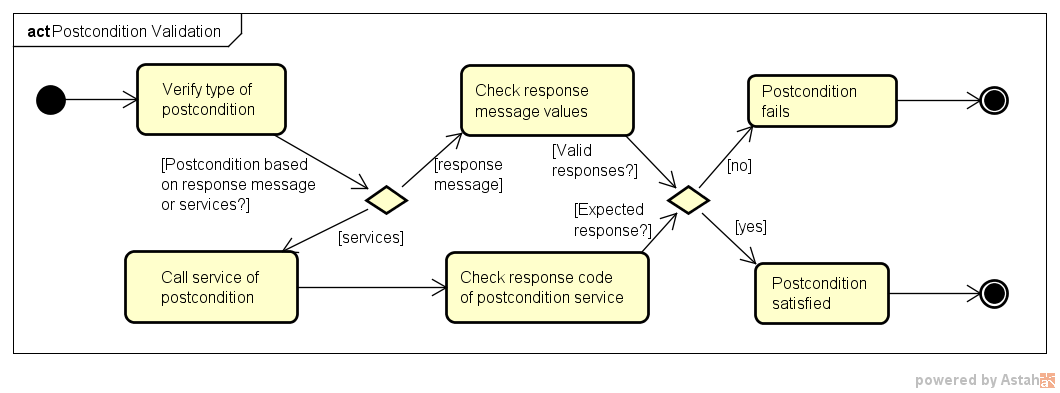
\includegraphics[width=\textwidth,trim = 0mm 5mm 0mm
0mm,clip]{PostconditionValidation.png} 
\vspace{-6mm}
\caption{Diagrama de atividades do processamento da pós-condição}
\label{FigServicePostcondition}
\end{figure}

A verificação das pós-condições acontece de modo muito similar a das
precondições. Há também os dois tipos, baseado em valores e em chamadas a
outros serviços. O diferencial está em que a validação dos valores passa a
ocorrer a partir dos valores contidos na mensagem de retorno. A Figura
\ref{FigServicePostcondition} descreve as etapas necessárias para validação de
cada precondição.


\section{EXTENSÃO DA NEOIDL PARA DESIGN BY CONTRACT}
\label{extensaoNeoIDL-DbC}

A sintaxe escolhida para possibilitar a especificação de pré e pós condições
na \neoidl{} foi influenciada por três linguagens e extensões de linguagens de
programação: Eiffel, JML e Spec\# (exemplificadas na subseção
\ref{implementDbC}). 

Em Eiffel, as asserções são expressões booleanas, de modo que uma pré e uma
poscondição podem ter resultado verdadeiro ou falso. As asserções também podem
incluir chamadas a funções, extendendo a validações a lógicas mais sofisticadas
\cite{meyer1992applying}. Essas caracteríticas, por serem simples e versáteis,
foram consideradas adequadas e incorporadas à especificação de
\designbycontract{} em contratos de serviços na \neoidl{}.

A primeira sintaxe de \designbycontract{} na \neoidl{} teve como
base a sintaxe da JML, especialmente em como se associar as pré e poscondições a
cada serviço ou capacidade, assemelhando-se a comentários e iniciados pelo
símbolo de arroba (@). A figura \ref{lst:precondicaoJML-neo} apresenta um
exemplo de especificação de precondição seguindo a linha da JML.

\vspace{6mm}

\begin{figure}[h]
\begin{small}
\lstinputlisting[language=NeoIDL,firstnumber=1]{DBCsimple.neo}
\vspace{-.5cm}
\end{small} 
\caption{Forma preliminar de precondição na \neoidl}
\label{lst:precondicaoJML-neo}
\end{figure}

Essa forma foi apresentada no Workshop de Teses e Dissertações do CBSoft em 2015
\cite{lima2015contratos}, ainda nos primeiros estágios do trabalho. Os revisores
apontaram dificuldade de distinguir, na especificação, entre as pré e
poscondições e os serviços e capacidades, pois possuiam prefixos muito
semelhantes (ver linhas 6 a 8).
Essas críticas impulsionaram a busca por outra sintaxe mais adequada aos elementos textuais já
existentes na \neoidl{}.

Spec\# possui uma forma de especificação de asserções em que as pré e
poscondições são declaradas logo após a assinatura do método ou classe, apenas
com o uso das palavras reservadas \emph{require} e \emph{ensure}, sem uso de
símbolos. Essa abordagem foi aplicada à \neoidl{} para versão final da sintaxe
com suporte a \designbycontract{}.

As próximas subseções apresentam alguns exemplos de especificação de pre e
poscondições na \neoidl{} e as mudanças introduzidas na sintaxe da linguagem.	


\subsection{Precondição básica}

\begin{figure}[htb]
\begin{small}
\lstinputlisting[language=NeoIDL,firstnumber=1]{DBCsimple.neo}
\end{small}
\caption{Exemplo da notação DBC básica na \neoidl{}}
\label{lst:DBCService}
\end{figure} 

\subsection{Pós-condição básica}

\ldots



\subsection{Precondição com chamada a serviço}

\begin{figure}[htb]
\begin{small}
\lstinputlisting[language=NeoIDL,firstnumber=1]{DBCservice.neo}
\end{small}
\caption{Exemplo da notação DBC na \neoidl{} com chamada a serviço}
\label{lst:DBCService}
\end{figure} 



\subsection{Pós-condição com chamada a serviço}

\ldots

\section{ESTUDO DE CASO: PLUGIN TWISTED}
\label{pluginTwisted}

\ldots

\subsection{Arquitetura}

% Diagrama da estrutura do código gerado


\subsection{Geração de código}

\section{ESTUDO EMPÍRICO DA ANÁLISE SUBJETIVA} 
\vspace{-6mm}

\label{analiseSubjetiva}
\vspace{-6mm}

%%%%
A language's expressiveness is the major criterion for choosing a language to
state a given set of facts: a language that cannot express the facts should not
be used. However, additional criteria are needed to choose among languages that
are sufficiently expressive  for a set of facts. Two of these criteria are how
ease it is to state the facts in the language and how easy is to perceive the
facts once they are stated.

expressividade de uma linguagem é o principal critério para a escolha de uma
linguagem para indicar um determinado conjunto de fatos: uma linguagem que não
podem expressar os fatos não devem ser usados. No entanto, os critérios
adicionais são necessários para escolher entre os idiomas que são
suficientemente expressivo para um conjunto de fatos. Dois desses critérios são
quão fácil é expor os fatos na linguagem e como é fácil de perceber os fatos,
uma vez que são demonstrados.

\cite{mackinlay1985expressiveness}

%%%%


%%%
Instead of aiming to be the best for solving any kind of
computing problem, DSLs aim to be particularly good for
solving a specific class of problems, and in doing so they
are often much more accessible to the general public than tra-
ditional programming languages.
\cite{taha2008domain}
%%%% 

%%%%
They offer substantial gains in expressiveness and ease of use compared
with GPLs in their domain of application’. [2] describes the typical costs of a
DSL, noting that a small extra initial investment in a DSL implementation typ-
ically leads to long term savings, in comparison to alternative routes.
\cite{tratt2008evolving}
%%%%

%%%%
A domain specific language (DSL) is a program-
ming language tailored for a particular application do-
main. Characteristic of an effective DSL is the ability
to develop complete application programs for a do-
main quickly and effectively. A DSL is not (neces-
sarily) “general purpose.” Rather, it should capture
precisely the semantics of an application domain, no
more and no less.

There are lots of advantages to using DSLs, start-
ing with the fact that programs are generally easier to
write, reason about, and modify compared to equivalent 
programs written in general purpose languages.
Indeed, these are the same advantages gained from using any high-level
programming language.
\cite{hudak1998modular}
%%%%




\subsection{Método}
\vspace{-6mm}

\subsection{GQM}
\vspace{-6mm}

\subsection{Questionário}
\vspace{-6mm}

\subsection{Análise dos Resultados}
\vspace{-6mm}


* Questionário montado para avaliar a utilidade de DbC com NeoIDL

* Inicialmente motivado pelo estudo do Alessandro Garcia

* GQM e Avaliação TAM

* Montagem do questionário

1. Perfil técnico-profissional do respondente
1.1 Para qual órgão ou empresa você presta serviços atualmente?
1.2 A quanto tempo você trabalha com desenvolvimento Web
1.3 A quanto tempo você desenvolve com uso de APIs Web (Web Service)
1.4 Qual o seu nível de experiência com especificação de API REST
1.5 Qual o seu nível de experiência com especificação de contratos com Swagger

3 Questões sobre especificação e implementação de APIs Web
3.1 A especificação do contrato formalmente, seja em Swagger ou NeoIDL, em
relação a descrição textual, aumentará meu nível de acerto na implementação (efetividade).
3.2 Identificar e compreender as operações e atributos na especificação Swagger
é simples para mim.
3.3 Identificar e compreender as operações e atributos na especificação NeoIDL é
simples para mim.

4. DbC
4.1 Conhecer previamente e explicitamente as precondições será útil para mim.
(Useful)
4.2 Aprender a identificar as precondições na NeoIDL parece ser simples pra mim
(Easy to learn)
4.3 Parece ser fácil para mim declarar uma precondição na NeoIDL
(Clear and understandable)
4.4 Me lembrar da sintaxe da precondição na NeoIDL é fácil  (Remember)

5. Geração de código
5.1 É claro e compreensível para mim o efeito da precondição sobre o código
gerado  (Controllable)
5.2 A geração do código de pré e pós-condições aumentará minha produtividade na
implementação do serviço (Job performance)
5.3 Assumindo ter a disposição a NeoIDL no meu trabalho, para especificação de
contratos e geração de código, eu presumo que a utilizarei regularmente no futuro.
5.4 Nesse mesmo contexto, eu vou preferir utilizar contratos escritos em NeoIDL
do que descritos de outra forma



* Distribuição do questionário

* Avaliação dos resultados

* Ameaças
- não foi fornecido nenhum material sobre a NeoIDL, apresentando somente o uma
descrição de serviço
- O questionário foi aplicado uma única vez, sem melhorias a partir do primeiro
conjunto de respostas


* Questionários futuros

A principal questão de pesquisa a ser avaliada com o uso do questionário é a utilidade em se agregar ao design das especificações de serviços REST as garantias de pré e
pós-condições. Em segundo momento, pressupondo a utilidade, avaliar se a NeoIDL
cumpre satisfatoriamente com este propósito, agregando à sintaxe da linguagem
a possibilidade de se expressar pré e pós-condições.

* Separar os respondentes em faixas de experiência. Verificar se as respostas
dos menos experientes precisam ser descartadas pela pouca capacidade crítica.
Separar a análise entre os respondentes que conhecem e os que não conhecem
Swagger.

* Perspectivas de comparação
a) Experiência com desenvolvimento com uso de REST
b) Experiência com Swagger
c) Utilidade da especificação formal de contratos
d) Percepção da NeoIDL sem DbC






% 5. Conclusão e trabalhos futuros
\chapter{CONCLUSÕES E TRABALHOS RELACIONADOS}
\vspace{-6mm}

\section{CONCLUSÕES GERAIS}
\vspace{-6mm}

A necessidade de estratégias de integração de sistemas e soluções adaptáveis às
constantes necessidade des mudanças tem levado às empresas a, cada vez mais,
adotarem o modelo de computação orientada a serviços -- SOC
\cite{papazoglou2008service} \cite{erl2009web}. A qualidade da especificação do
serviço por meio de seu contrato é um dos fatores determinantes para o sucesso
do uso de SOC.


A boa definição dos contratos \ldots 
\vspace{-6mm}


-- Usar na motivação --
The problem gets aggravated by
the fact that modern software applications are expected to
make use of these reusable modules as much as possible,
in an effort to reduce both the development costs and the
production time. Unfortunately, this situation opens the door
for the propagation of security vulnerabilities among several
applications as a result of the incorrect enforcement of security
properties in reusable software modules and threatens the
security and safety of applications as a whole.
\cite{rubio2013verifying}

Meyerovich e Rabkin \cite{meyerovich2013empirical} analisaram quase 800.000
projetos de código aberto para tentar identificar o que leva a escolha de uma
linguagem em detrimento de outra. Eles concluíram que o domínio em que a
linguagem será aplicada, ou seja, o problema que ela pretende resolver, tem mais
influência que a similaridade semântica com outras linguagens já utilizadas. 
\cite{meyerovich2013empirical}





\section{TRABALHOS RELACIONADOS E PESQUISAS FUTURAS }
\vspace{-6mm}

\ldots

- Trabalhos relacionados com hipermedia




\clearpage
\newpage
%%%%%%%%%%%%%%%%%%%%%%%% Bibliografia %%%%%%%%%%%%%%%%%%%%%%%

%Espa�amento simples
%\baselineskip=12pt

% espa�amento 1,5
\linespread{1.3}

 \bibliographystyle{plainbr}

%\bibliographystyle{ieee}

\addcontentsline{toc}{chapter}{REFERÊNCIAS BIBLIOGRÁFICAS}

\bibliography{bibdata}

%%%%%%%%%%%%%%
% \input{biblio}

\baselineskip=18pt
%%%%%%%%%%%%%%%%%%%%%%%%% Ap�ndices
\appendix



\clearpage

\addcontentsline{toc}{chapter}{APÊNDICES}
\hspace{1mm}

\vfill

\begin{large}

\begin{center}
\begin{bf}
APÊNDICES

% T�TULO DO PRIMEIRO CAP�TULO DO AP�NDICE

\end{bf}
\end{center}
\end{large}

\vfill

\clearpage
% 

\chapter{TRANFORMAÇÃO SWAGGER PARA NEOIDL}
\label{scriptSwagger2NeoIDL}
\vspace{-6mm}

\begin{figure}[h]
\begin{small}
\lstinputlisting[language=Perl,firstnumber=1]{swagger2NeoIDL.pl}
\vspace{-.5cm}
\end{small}
\caption{Conversor de Swagger para \neoidl{}}
\label{lst:swagger2NeoIDL}
\end{figure}

\ldots 

% \chapter{ESTRUTURA DA LINGUAGEM NEOIDL}
\label{apend:estruturaLexicaNeoIDL}

Estas informações foram geradas automaticamente pelo BNF-Converter \cite{forsberg-bnfc:2004}
\textit{parser generator}) a partir da gramática da \neoidl{}.

\section{ESTRUTURA LÉXICA DA NEOIDL}

\begin{enumerate}
  \item Identificadores
  
  Identificadores \nonterminal{Ident} são literais (\textit{strings}) não
  delimitados que começam com uma letra seguida por letras, números e os
  caracteres {\tt \_ '}, exceto palavras reservadas.
  
  \item Literais
  
  Literais de texto são cadeias de caracteres  \nonterminal{String}\ com a forma
  \terminal{``}$x$\terminal{``}, onde $x$ é qualquer sequencia de caracter,
  exceto \terminal{``}, a menos que precedido por \text{\tt \char92{}}.
  
  Literais numéricos \nonterminal{Int}\ são sequências não vazias de números.
  
  Literais de ponto flutuantes \nonterminal{Double}\ tem a estrutura
  definida pela seguinte expressão regular: $\nonterminal{digit}+ \mbox{{\it
  `.'}} \nonterminal{digit}+ (\mbox{{\it `e'}} \mbox{{\it `-'}}?
  \nonterminal{digit}+)?$, ou seja, duas sequências de números separadas por um
  ponto, opcionalmente precedida de um símbolo de negativo.

  \item Palavras reservadas e símbolos

  O conjunto de palavras reservadas são os terminais da gramática da linguagem
  \neoidl{}. As palavras reservadas não compostas de letras são chamados
  símbolos, que são tratados de forma diferente dos identificadores. A
  sintaxe analisador léxico segue regras típicas de linguagens como Haskell, C e
  Java, incluindo correspondência mais longa e convenções para o espaço.
  
  As palavras reservadas utilizadas na \neoidl{} são as seguintes: \\

\begin{tabular}{lll}
{\reserved{annotation}} &{\reserved{call}} &{\reserved{entity}} \\
{\reserved{enum}} &{\reserved{extends}} &{\reserved{float}} \\
{\reserved{for}} &{\reserved{import}} &{\reserved{int}} \\
{\reserved{module}} &{\reserved{path}} &{\reserved{resource}} \\
{\reserved{string}} & & \\
\end{tabular}\\
  
Os símbolos utilizados na \neoidl{} são os seguintes: \\

\begin{tabular}{lll}
{\symb{\{}} &{\symb{\}}} &{\symb{;}} \\
{\symb{{$=$}}} &{\symb{.}} &{\symb{@}} \\
{\symb{(}} &{\symb{)}} &{\symb{0}} \\
{\symb{{$=$}{$=$}}} &{\symb{{$<$}{$>$}}} &{\symb{{$>$}}} \\
{\symb{{$>$}{$=$}}} &{\symb{{$<$}}} &{\symb{{$<$}{$=$}}} \\
{\symb{[}} &{\symb{]}} &{\symb{@get}} \\
{\symb{@post}} &{\symb{@put}} &{\symb{@delete}} \\
{\symb{/@require}} &{\symb{/@ensure}} &{\symb{/@invariant}} \\
{\symb{/@otherwise}} &{\symb{/**}} &{\symb{*/}} \\
{\symb{*}} &{\symb{@desc}} &{\symb{@param}} \\
{\symb{@consume}} &{\symb{,}} & \\
\end{tabular}\\

\end{enumerate}

\section{ESTRUTURA SINTÁTICA DA NEOIDL}\label{sub:sintatico}

Não-terminais são delimitados entre $\langle$ e $\rangle$. O símbolo {\arrow}
(produto), {\delimit} (união) e {\emptyP} (regra vazia) advêm da notação BNF.
Todos os demais símbolos são terminais.\\


\begin{small}

\begin{tabular}{lll}
\label{lst:BNFnot}
{\nonterminal{Modulo}} {\arrow} {\terminal{module}} {\nonterminal{Ident}} {\terminal{\{}} \\ 
 \quad {\nonterminal{ListImport}} \\ 
 \quad {\nonterminal{MPath}} \\ 
 \quad {\nonterminal{ListEnum}} \\ 
 \quad {\nonterminal{ListEntity}} \\ 
 \quad {\nonterminal{ListResource}} \\ 
 \quad {\nonterminal{ListDecAnnotation}} \\ 
{\terminal{\}}}  \\
\end{tabular}


\begin{tabular}{lll}
{\nonterminal{Import}} & {\arrow}  &{\terminal{import}} {\nonterminal{NImport}} {\terminal{;}}  \\
\end{tabular}

\begin{tabular}{lll}
{\nonterminal{MPath}} & {\arrow}  &{\emptyP} \\
 & {\delimit}  &{\terminal{path}} {\terminal{{$=$}}} {\nonterminal{String}} {\terminal{;}}  \\
\end{tabular}

\begin{tabular}{lll}
{\nonterminal{NImport}} & {\arrow}  &{\nonterminal{Ident}}  \\
 & {\delimit}  &{\nonterminal{Ident}} {\terminal{.}} {\nonterminal{NImport}}  \\
\end{tabular}

\begin{tabular}{lll}
{\nonterminal{Entity}} & {\arrow}  &{\nonterminal{ListDefAnnotation}} {\terminal{entity}} {\nonterminal{Ident}} {\terminal{\{}} {\nonterminal{ListProperty}} {\terminal{\}}} {\terminal{;}}  \\
 & {\delimit}  &{\nonterminal{ListDefAnnotation}} {\terminal{entity}} {\nonterminal{Ident}} {\terminal{extends}} {\nonterminal{Ident}} {\terminal{\{}} {\nonterminal{ListProperty}} {\terminal{\}}} {\terminal{;}}  \\
\end{tabular}

\begin{tabular}{lll}
{\nonterminal{Enum}} & {\arrow}  &{\terminal{enum}} {\nonterminal{Ident}} {\terminal{\{}} {\nonterminal{ListValue}} {\terminal{\}}} {\terminal{;}}  \\
\end{tabular}

\begin{tabular}{lll}
{\nonterminal{DecAnnotation}} & {\arrow}  &{\terminal{annotation}} {\nonterminal{Ident}} {\terminal{for}} {\nonterminal{AnnotationType}} {\terminal{\{}} {\nonterminal{ListProperty}} {\terminal{\}}} {\terminal{;}}  \\
\end{tabular}

\begin{tabular}{lll}
{\nonterminal{DefAnnotation}} & {\arrow}  &{\terminal{@}} {\nonterminal{Ident}} {\terminal{(}} {\nonterminal{ListAssignment}} {\terminal{)}} {\terminal{;}}  \\
\end{tabular}

\begin{tabular}{lll}
{\nonterminal{Parameter}} & {\arrow}  &{\nonterminal{Type}} {\nonterminal{Ident}} {\nonterminal{Modifier}}  \\
\end{tabular}

\begin{tabular}{lll}
{\nonterminal{Assignment}} & {\arrow}  &{\nonterminal{Ident}} {\terminal{{$=$}}} {\nonterminal{Value}}  \\
\end{tabular}

\begin{tabular}{lll}
{\nonterminal{Modifier}} & {\arrow}  &{\emptyP} \\
 & {\delimit}  &{\terminal{{$=$}}} {\terminal{0}}  \\
\end{tabular}

\begin{tabular}{lllllllll}
{\nonterminal{AnnotationType}} & {\arrow}  &{\terminal{resource}}  
 & {\delimit}  &{\terminal{enum}}  
 & {\delimit}  &{\terminal{entity}}  
 & {\delimit}  &{\terminal{module}} 
\end{tabular}

\begin{tabular}{lll}
{\nonterminal{Resource}} & {\arrow}  &{\nonterminal{ListDefAnnotation}} {\terminal{resource}} {\nonterminal{Ident}} {\terminal{\{}} {\terminal{path}} {\terminal{{$=$}}} {\nonterminal{String}} {\terminal{;}} {\nonterminal{ListCapacity}} {\terminal{\}}} {\terminal{;}}  \\
\end{tabular}

\begin{tabular}{lll}
{\nonterminal{Capacity}} & {\arrow}  &{\nonterminal{NeoDoc}} {\nonterminal{ListDefNAnnotation}} {\nonterminal{Method}} {\nonterminal{Type}} {\nonterminal{Ident}} {\terminal{(}} {\nonterminal{ListParameter}} {\terminal{)}} {\terminal{;}}  \\
\end{tabular}

\begin{tabular}{lllllllll}
{\nonterminal{Method}} & {\arrow}  &{\terminal{@get}} 
 & {\delimit}  &{\terminal{@post}} 
 & {\delimit}  &{\terminal{@put}}  
 & {\delimit}  &{\terminal{@delete}} 
\end{tabular}\\
\end{small}    
% \chapter{CLASSES DO PACOTE DBCCONDITIONS}
\label{classesDbcCondition} 
\vspace{-6mm}

\begin{small}
\scriptsize
\lstinputlisting[language=PythonTwisted,firstnumber=1]{trechos_codigo/dbcCondition.py}
\end{small}

% fim do texto


\end{document}
